%%%%%%%%%%%%%%%%%%%%%%%%%%%%%%%%%%%%%%%%%%%%%%%%%%%%%%%%%%%%%%%%%%%%%%%%%%%%%
%%%% Preamble
%%%%%%%%%%%%%%%%%%%%%%%%%%%%%%%%%%%%%%%%%%%%%%%%%%%%%%%%%%%%%%%%%%%%%%%%%%%%%

%%%% The uwthesis.sty file relies on the memoir class!
%%%% You should be using the memoir class anyway; it makes life easier:
%%%% http://www.ctan.org/tex-archive/macros/latex/contrib/memoir/
\documentclass[oneside, letterpaper, 12pt, oldfontcommands]{memoir}

%%%% Import uwthesis.sty to get official formatting, then set your variables.
\usepackage{uwthesis}

\settitle{Measurement of Electroweak WZ Production and Search for New Physics in Proton--Proton Collisions at $\sqrt{s} = 13$ TeV with the CMS Detector at the CERN LHC}
\setauthor{Kenneth Long}
\setdepartment{Physics}
\doctors % or \masters
\setgraddate{2018}
\setdefensedate{15 Dec. 2018} % or whatever format you want

%%%% Members of the Final Oral Committee (FOC)
%%%% Give name, rank, and department
%%%% 
\setfoca{Matthew Herndon}{Professor}{Physics} % <- Your advisor
\setfocb{John Adams}{Professor}{Physics}
\setfocc{Thomas Jefferson}{Assistant Professor}{Physics}
\setfocd{James Madison}{Professor}{Physics}
\setfoce{James Monroe}{Professor}{Materials Engineering}
\setfocf{Grover Cleveland}{Professor}{Zoology}

%%%% Your abstract, used for the UMI abstract and in your front matter
\setabstract{%
}

%%%%%%%%%%%%%%%%%%%%%%%%%%%%%%%%%%%%%%%%%%%%%%%%%%%%%%%%%%%%%%%%%%%%%%%%%%%%%
%%%% Document
%%%%%%%%%%%%%%%%%%%%%%%%%%%%%%%%%%%%%%%%%%%%%%%%%%%%%%%%%%%%%%%%%%%%%%%%%%%%%

\begin{document}

% Tell the memoir class to set up lowercase roman for pagination, etc.
\frontmatter

%%%% Uncomment this to create a UMI abstract page.
%%%% If you are submitting electronically, however, this page is unnecessary.
% \theumiabstract

% The title page
\thetitlepage
\clearpage

% The copyright page, if you want to pay the fee and register copyright.
\thecopyrightpage
\cleardoublepage

% These above pages should not be counted, so we reset the counter to 1.
\setcounter{page}{1}

% An abstract may be required by your department.
\section{Abstract}
\uwabstract
\cleardoublepage

% Acknowledgements go here if you want to include them.
\section{Dedication}
This thesis is dedicated to the memory of Dr. David Murdock, whose
passion for physics and education helped countless students
at Tennessee Technological University and far beyond. Your love of
particle physics spread to me, and your generosity with your time and knowledge
gave me the tools to be successful beyond the walls of Tennessee Tech.
\clearpage
% Acknowledgements go here if you want to include them.
\section{Acknowledgements}
This thesis is dedicated to the memory of Dr. David Murdock, whose
passion for physics and education helped countless students
at Tennessee Technological University and far beyond. Your love of
particle physics spread to me, and your generosity with your time and knowledge
gave me the tools to be successful beyond the walls of Tennessee Tech.
\clearpage

% Table of contents
\maxtocdepth{subsection}
\tableofcontents* % the * means that there isn't an entry for the TOC itself
% \clearpage
% \listoffigures  % if you have any figures
% \clearpage
% \listoftables   % if you have any tables

% Tell the memoir class to set up normal pagination, etc. for the main doc
\mainmatter

\chapter{Introduction}
\label{ch:introduction}

This thesis presents measurements of the production of events with
three leptons, two forward ``jets'' of clustered hadronic particles,
with an imbalance of transverse momentum. 
Events are selected to isolate contributions involving the simultaneous
production of a $\PW^{+}$ or $\PW^{-}$ and $\PZ$ boson, the heavy particles
that communicate the weak force.
Selected events are used
to measure the rate of production of processes predicted by the standard
model (SM) of particle physics, the most complete theoretical expression
of the known particles and forces of the universe, and to search for hypothetical extension
of the SM. 

A dedicated search
for a rare, previously unobserved, SM process, referred to as electroweak
WZ (\EWWZ) production, is presented. 
The presence and production rate of the \EWWZ process is intimately connected to the 
phenomenon of EW symmetry breaking (EWSB) \cite{Quigg:2009vq}, which leads to 
the W and Z bosons acquiring masses
and self-interactions. A fundamental prediction
of EWSB, fulfilled in the standard model (SM) by the Brout-Englert-Higgs (BEH) mechanism,
is the emergence of a scalar particle, known 
to as the Higgs boson. 
This particle was first observed by the 
ATLAS~\cite{Aad:2012tfa} and CMS~\cite{Chatrchyan:2012xdj,Chatrchyan:2013lba} Collaborations
at CERN in 2012, providing compelling evidence for the BEH mechanism as
a component of the SM theory.

In addition, constraints on physics beyond the SM (BSM) are placed on in terms
of explicit models predicting charged Higgs bosons decaying to a $\Wpm$ and a $\PZ$
boson, and on

\section{The universe of particles}

The idea of understanding the physical world by identifying its
fundamental constituents is a very old one. Ancient eastern and
western philosophers independently attempted the feat, concluding
that the world could be reduced 
to ``elements'' such as water, earth, and fire.
As observational science became a more prominent component of modern thought, 
evidence mounted that these elements themselves were 
not indivisible. Perhaps the Greeks had not identified
the correct fundamental elements, but the belief that this endeavor could
be accomplished lived on.

A major attraction of identifying the fundamental building blocks of the universe
is the implication for constructing a macroscopic description from these
pieces. This process of understanding a complex system 
by reducing it to its essential components
termed ``reductionism'' by philosophers, 
has formed the backbone of scientific endeavor for much of history.
In practice, the step from the fundamental to the macroscopic 
is far from trivial. Despite a well-established
understanding of the proton constituents and their interactions,
predicting the proton mass from first principles has only recently 
been achieved~\cite{Durr:2008zz}, and larger systems remain well
out of reach.
In addition to the challenges of calculability, additional structures
may arise from the nature of large systems, such as ferromagnetism or 
superconductivity.
This long-accepted path to a complete description of the physical world
has thus been called into question, and it may never be feasible
to achieve a theory of biology built from the findings of particle 
physics~\cite{Anderson393}.
Yet there is an undeniable elegance in achieving a concise description
of the fundamental elements of the natural world and their interactions,
and this remains the target of the field of particle physics today. 

The modern genesis of the field can perhaps be credited to 
the discovery of the electron in 1897 by J. J. Thomson, a particle still
believed to be elementary today.
Further experiments showed that the electron carries the smallest quantity of electric charge found
freely in nature, and we now know that many macroscopic electrical phenomena
arise from the motion of electrons in atoms.
A mathematical understanding of these electromagnetic interactions had 
already been established by James Clerk Maxwell decades before Thompson's work
The idea of a particle of light is therefore seemingly at odds with Maxwell's theory,
which described light as a oscillations of electromagnetic fields,
but a quanta of light was central to the explanation of black-body radiation provided by Max Planck 
and for the theoretical explanation of the photoelectric effect developed by Albert Einstein.
The theory of fields and particle-like characteristics of electromagnetic
interactions were reconciled shortly after these proposals by the 
rapidly-developing quantum theory.
The quanta of light, the photon, is now understood to communicate the electromagnetic force.
By the early 1940s, these pieces had evolved into the theory of quantum 
electrodynamics, the first
quantized theory of particles and their interactions in the language 
of quantum field theory. 

Simultaneous to the efforts to develop a mathematical language to describe 
the fundamental particles and their interactions was an experimental effort 
to find and categorize them. New equipment for detecting these particles,
such as the cloud chamber developed by Charles Wilson, 
gave a perspective on the spontaneous 
decay of atoms and opened our eyes to the radiation bombarding the earth from
outside the atmosphere. By the 1950s, particle physicists were faced with a ``particle zoo''
of seemingly fundamental objects spanning a huge range of masses. 
An underlying structure of the properties of many of these particles, 
now known as hadrons, was described by Murray Gell-Man and George Zweig in 1964.
They realized the properties of the many observed hadrons could be 
attributed to combinations of different elementary particles,
which Gell-Man termed quarks.
Whether these particles were physical entities or abstractions was 
not immediately evident, but experiments at the Stanford Linear Accelerator
at the end of the 1960s showed the proton to have point-like constituents
with the properties Gell-Man and Zweig predicted.

Despite the progress in explaining the structure of hadronic matter,
it remained unclear that the language of a quantum gauge theory, 
so successful in the formulation of the electromagnetic interaction, could 
also describe the strong nuclear force responsible for the formation
of these composite particles, and the weak nuclear force responsible for
a subset of their decays. Both exhibited striking differences with
respect to the electromagnetic interaction:
the weak nuclear force acts over a much smaller distance, while
the strong nuclear 
force has an inverted scaling with distance, increasing at higher separation
of the interacting objects while decreasing at very short ranges. 

A unification of the electromagnetic and weak nuclear force was achieved
by Sheldon Glashow, Abdus Salam, and Steven Weinberg in the early 1970s.
A crucial component of their theory is the presence of a scalar field, 
which gives mass to the W and Z bosons through EWSB, leading to the 
short range of the weak force.
A description of the strong nuclear force as a quantum 
gauge theory followed,
with the inverse distance scaling properties of the theory,
termed quantum chromodynamics (QCD), demonstrated by
David Gross, David Politzer and Frank Wilczek.
The discovery of the gluon, the so-called gauge boson of the theory,
in 1979 at the Deutsches Elektronen-Synchrotron (DESY) in Hamburg, Germany
provided definitive confirmation
of gauge theory as the theoretical foundation of the particle physics.
The outstanding prediction of the 
electroweak theory, that the W and Z bosons which communicate the weak 
interaction acquire mass through the presence of scalar field, required
longer for experimental confirmation. This confirmation arrived a half-century
later, with the observation of the Higgs boson at CERN in 2012.
Together, the description of these interactions and the particle content
and these interactions described by the EW and QCD theories are known
as the standard model of particle physics.

\begin{figure}[htbp]
  \centering
   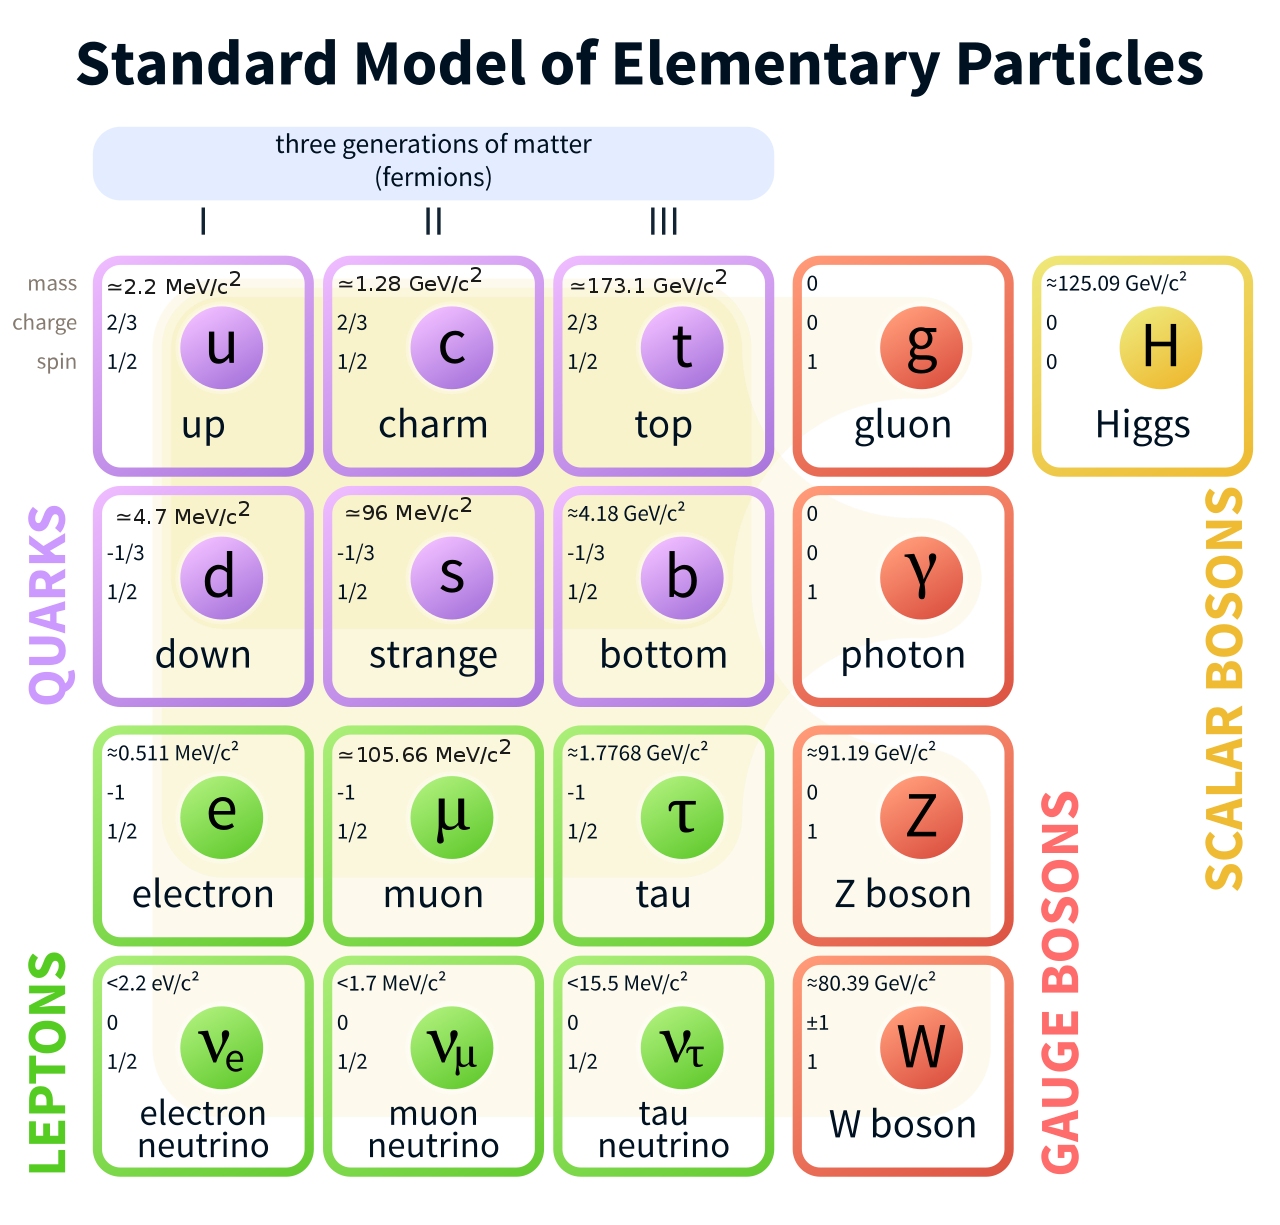
\includegraphics[width=0.9\textwidth]{figures/Chapter1/ChartOfParticles.png}
  \caption{
    The experimentally established particle content of the universe.
  }
 \label{fig:theparticles}
\end{figure}

The currently known particle content of the universe is depicted in Fig.~\ref{fig:theparticles}.
The quarks, highlighted in green, and leptons, highlighted in purple,
form matter, while the vector bosons, highlighted in red, mediate the 
interactions of this matter. The Higgs particle, shown in yellow,
has a unique role in the SM. It arises from the Higgs field, which
leads to masses for the W and Z bosons as well as the quarks and leptons.
The underlying mathematical framework used to understand the quantum 
properties of these particles and their interactions will be further discussed
in Chapter~2. 

\textbf{Go ahead and expand the description of what the particles are in this section}.

\section{Particle collider experiments}
\textbf{Introduce idea of scattering experiment}
\textbf{Introduce idea of cross section}

To observe the smallest pieces of matter, one must break matter into pieces.
The discovery of radioactivity in the late 1800s by Henri Becquerel had
profound implications for this idea, as it represented the spontaneous
disintegration of atoms. 
In addition to studying the products of these decays themselves, 
Earnest Rutherford realized the energetic decay products could be used
to perform the first particle scattering experiments. By directing the 
helium nuclei emitted from radioactive radium decay towards gold foil
and measuring the deflection
angles, he and his collaborators established the existence of the atomic nuclei.
Inferring information about the properties and interactions of particles based on their
behaviour when scattered is still central to particle physics experiment today.

Rutherford continued to use the radioactive decays of elements as a means
for particle acceleration in the early 1900s. Yet it was clear that
a means of accelerating collisions to higher energies would be needed
to continue to probe the structure of the nucleus.
These efforst lead to the invention of the 
the first particle accelerators, which have come to define the field ever since.
An electrostatic accelerator was developed at the Cavendish Laboratory
in Cambridge, England by John Crockhoff and Ernest Walton and
was used to split Lithium into Helium atoms in 1932.
Concurrently, Ernest Lawrence developed the cyclotron in California,
which became a model for many future accelerator facilities.

These inventions triggered an explosion in the field, marked by a continual 
effort to collide particles at higher and higher energies. Many major discoveries
are closely linked with technological advancements or collaborative
efforts leading to more powerful accelerators.
The facilities at the European Center for Nuclear
Research (CERN), DESY, and at the 
Fermi National Accelerator Laboratory (Fermilab) in Illinois
are strongly associated with the 
discoveries they enabled, including evidence for the force carries
of the EW and QCD interactions, the W and Z bosons and the gluon.

The most powerful collider ever built, the LHC at CERN,
now allows the study of the most energetic particle collisions ever
recorded in the laboratory, reaching concentrated energies only replicated
in the most cataclysmic events in the universe. The LHC
was planned, developed, and built over the course of decades, with
personnel and funding from countries throughout the world.
This work is based on studies of pp collisions delivered by the LHC 
and collected by the Compact Muon Solenoid detector in 2016.

\textbf{Maybe explain a bit more what a scattering experiment is here}

The LHC and Compact Muon Solenoid detector are discussed in detail 
in Chapter~3 of this thesis.

\section{Motivation and context of this result}
The work presented in this thesis
has two related motivations: performing a measurement of a rare
process predicted by the SM, and searching for signs of 
BSM physics in a channel and topology sensitive to modifications of
the EW sector of the SM.
Characterizing the self-interactions of the vector bosons is an important
step to understanding the self-consistency of the SM, and a useful probe
of possible deviations from its predictions. Because the production of events
with multiple vector bosons in the final state
requires collisions with a high center of mass energy, the LHC has
the potential to explore these states in more depth 
than previously achieved.

Measurements of WW and WW$\gamma$ production in electron--positron collisions
were first made at the LEP
Collider at CERN by the ALEPH, DELPHI, L3, and OPAL Collaborations~\cite{LEP-2}.
These processes are sensitive to the triple vector boson couplings
WWZ and WW$\gamma$, and the quartic couplings WW$\gamma\gamma$
and WWZ$\gamma$. The production rate and angular distributions of the decay
products of the vector bosons in these states were used to derive values 
of the triple and quartic couplings. No deviations were observed from the 
predictions of the SM with a light Higgs boson.

Production of charged vector boson pairs was also studied in proton--antiproton
collisions at the Tevatron Collider at the Fermilab. 
The measurement of WZ production, inclusive in the
number of clustered hadronic particles -- referred to as jets (j), was
first performed by the CDF~\cite{Aaltonen:2012vu,Abulencia:2007tu} 
and D0~\cite{Abazov:2012cj} Collaborations at the Tevatron in 2006. 
Measurements of the WWZ coupling were found to be consistent with the results
from the LEP experiments and with the SM.

Experimental sensitivity to quartic couplings of the massive vector boson 
was first achieved at the LHC.
In pp collisions, quartic WZ interactions are accessible through triple 
vector boson production or through vector boson scattering (VBS), 
in which vector bosons are radiated from the quarks in the colliding protons 
before interacting.
These interactions include WZ quartic couplings, as shown in Fig.~\ref{fig:feynmanDiagrams}~(a). 
Constraints on the deviations of quartic couplings from the SM prediction, 
referred to as anomalous quartic gauge couplings (aQGC), in 
WZ events with at least two jets (\WZjj) were first
presented by the ATLAS collaboration at 8 TeV~\cite{Aad:2016ett}. This result
is the first study of WZ vector boson scattering at CMS. 

\begin{figure}[htbp]
  \centering
   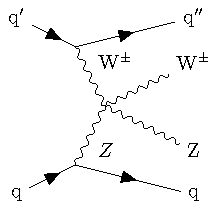
\includegraphics[page=1,width=0.25\textwidth]{figures/FeynmanDiagrams/feynmanVBS.pdf}
   \includegraphics[page=2,width=0.25\textwidth]{figures/FeynmanDiagrams/feynmanVBS.pdf}
   \includegraphics[page=3,width=0.25\textwidth]{figures/FeynmanDiagrams/feynmanVBS.pdf}
  \caption{Representative Feynman diagrams for \WZjj production in the SM and BSM. 
  EW-induced WZ production includes quartic interactions (a) of the vector bosons.
  New physics in the EW sector modifying the quartic coupling 
  can be parameterized in terms of dimension-eight effective field theory operators (b).
  Specific models modifying this interaction include those predicting charged Higgs bosons (c).
  }
 \label{fig:feynmanDiagrams}
\end{figure}

A well-motivated modification of the WWZZ quartic coupling would arise from
the presence of charged Higgs bosons.
In the SM, EWSB is fulfilled by a single Higgs field, which transforms as an SU(2) doublet.
Extending the Higgs sector by at least one additional SU(2) doublet or triplet leads necessarily
to additional charged scalar particles~\cite{Arbey:2017gmh}. An extended Higgs sector is predicted by many
complex BSM theories, including the Minimal Supersymmetric SM. 
Even without an 
underlying theory predicting an extended Higgs sector, establishing if the Higgs 
sector is more complex than the simplest fulfillment of the BEH mechanism is of 
great interest.

Extensive searches for charged Higgs bosons were carried out at the 
LEP Collider~\cite{ALEPHCollaboration2013}. 
These searches placed strong constraints on the production
and decay of charged Higgs bosons in scenarios such as the MSSM, where leptonic
decays are favored. 
The \WZjj channel is particularly useful as a search for Higgs particles 
which couple only to the vector bosons, such as those predicted in the 
Georgi-Macacheck model~\cite{Georgi:1985nv}. In this case, production via WZ vector
boson fusion, as shown in Fig.~\ref{fig:feynmanDiagrams} (c) is the dominant 
production mode.
The ATLAS Collaboration first studied charged Higgs production in this channel
at 8 TeV~\cite{Aad:2015nfa}, using events with one boson decaying hadronically.
CMS and ATLAS have performed searches for charged Higgs production in this channel 
at 13 TeV~\cite{Sirunyan:2017sbn,Aaboud:2018ohp}. This analysis extends the previous result from CMS and is complementary
to the recent ATLAS result.

\section{Overview}

The outline of this work is as follows: Chapter~2 presents an extended 
overview of the theoretical underpinnings of this work, including the foundations
of the SM and the role of \EWWZ production in this framework. The motivations 
and structure of SM extensions probed in this work are also introduced.
Chapter~3 introduces the experimental setup and apparatus used to study W and 
Z boson production in the laboratory. The LHC and the Compact Muon Solenoid 
detector are presented and discussed. Chapter~4 describes the procedure of 
building predictions for vector boson production in pp collisions.
The use of these predictions in interpreting results, and in developing simulation
of particle production and decays in pp collisions including their interactions
with the detector -- which are used 
guide the analysis approach and optimizations -- are discussed. Chapter~5 presents
the process of finding particle candidates from electronic signals in the detector.
Chapter~6 details the procedure of this analysis and the statistical underpinnings
used to extract results. Chapter~7 discusses the results obtained from this study
including interpretations and implications. Chapter~8 summarizes the
results presented and discusses future extensions.

\chapter{Vector boson scattering in the standard model and beyond}
\label{ch:phenomenology}

\section{Mathematical formalism of the standard model}
\label{sec:formalism}

Guided by experimental tests and
discoveries, we have built a description of all the known interactions 
of the SM particles in the language of gauge quantum field theory (QFT).
An in-depth discussion of QFT and the mathematical expression of the SM is
the subject of many textbooks, e.g., 
Refs.~\cite{Aitchison:2003tq,Srednicki:2007qs,Peskin:1995ev,Halzen:1984mc,Barger:1987nn}. 
An overview of the ideas
most central to this thesis is presented here, following the discussion
of Refs.~\cite{Quigg:2009vq,Peskin:1995ev}.

Particles in QFT arise as excitations in quantum fields.
The equations of motion and interactions for the quantum fields of the SM can
be extracted from the SM Lagrangian, which can be divided into 
terms governing the propagation of the free fields of the spin $1/2$ 
fermions (quarks and leptons), the spin 0 Higgs field, and the vector boson fields:
\begin{equation}
  \mathcal{L}_{SM} = \mathcal{L}_{\text{gauge}} + \mathcal{L}_{\text{leptons}} + 
      \mathcal{L}_{\text{quarks}} + \mathcal{L}_{\text{scalar}} \,.
  \label{eq:smlagrangian}
\end{equation}
In this expression, $\mathcal{L}_{\text{gauge}}$ is a function of the 
spin 1 vector fields.
The $\mathcal{L}_{\text{quark}}$ term includes kinetic terms describing the 
propagation of free quarks as well as interaction terms coupling the quarks
the vector fields
The term $\mathcal{L}_{\text{leptons}}$ is built from similar kinetic terms and 
interaction terms coupling the leptons to the electroweak fields, reflecting
the fact that the leptons do not participate in the strong interaction.
For free fields fermions $\psi$, the kinetic terms of the Lagrangian are defined as
\begin{equation}
  \mathcal{L} = \bar{\psi}(i\gamma^{\mu}\partial_\mu - m)\psi
  \label{eq:freeFermion}
\end{equation}
where $\psi$ is the spinor fermion field, $\gamma^{\mu}$ are the 
Dirac (or $\gamma$) matrices, and $m$ is the mass of the fermion. 
The equations of motion derived from this expression give the well-known
Dirac equation.

A fundamental property of the SM Lagrangian is its invariance 
under under a class of transformations known as ``gauge transformations.'' 
The vector fields $A^{a}_\mu$ are referred to as \emph{gauge fields}
because of their role in ensuring that the Lagrangian remains invariant
under a particular transformation, which may be respected by subsets of the 
fermionic fields.
A gauge transformation is ``generated''
by the Lie group defined by a set of $n\times n$ matrices $t^{a}$.
Infinitesimal unitary rotations of the fields of the form $\exp{(iV(x))}$,
for an arbitrary $n\times n$ matrix $V(x)$ in the group, can be expressed
in terms of the $t^{a}$ matrices and an arbitrary function $\alpha(x)$ as
$V(x) =1 + i\alpha^{a}(x)t^{a}+\mathcal{O}(\alpha^{2})$. Under this rotation,
a gauge field transforms as
\begin{equation}
  A^{a}_\mu \rightarrow A^{a}_\mu + \frac{1}{g}\partial_\mu^{a} + f^{abc}A_\mu^{b}\alpha^{c} \,.
  \label{eq:covariantDeriv}
\end{equation}
Here $g$ is the coupling constant of the theory
and $f^{abc}$ are the \emph{structure constants} of the transformation, related
to the commutator of the generating matrices as $[t^{a}, t^{b}] = if^{abc}t^{c}$.
By introducing the \emph{covariant derivative} $D_\mu$ associated with the gauge field $A_\mu$,
\begin{equation}
  D_\mu = \partial_\mu - igA_\mu^{a}t^{a} \,.
\end{equation}
and promoting the partial derivative of the Lagrangian in Equation~\ref{eq:freeFermion},
to a covariant derivative, the expression is naturally invariant under these transformations.
Futhermore, the expression has further given rise to interactions between the fermion fields
and the gauge fields. In this way, we conclude that the interactions of the fermions
with the vector bosons arise as a consequence of the gauge symmetry of the theory.

The full SM Lagrangian respects transformations of the
group $\SUthree_C \times\SUtwo_L\times \Uone_Y$. 
In this expression, $\SUthree$ ($\SUtwo$) is the Lie group of all unitary two-by-two
(three-by-three) matrices with determinant 1, and $\Uone$ is the Lie group
of complex numbers. The subscripts $C$, $L$, and $Y$ indicate the fermion
and gauge fields that are impacted by the rotation: the $\SUthree$ transformation
concerns only objects with color charge (quarks and gluons), and the $\SUtwo$
and $\Uone$ rotations concern weak isospin charge, carried only by 
the left-handed fermions, and weak hypercharge.
The measurements in this thesis are probe the structure of the 
electroweak force, so it is instructive to consider this in more detail.

The left-handed leptons form doublets under the $\SUtwo$ isospin rotation:
\begin{equation}
  L_\ell = 
  \begin{pmatrix}
      \PGn \\
      \ell^{-}
  \end{pmatrix}_{L} \,.
\end{equation}
A similar expression holds for the quarks:
\begin{equation}
  L_q = 
  \begin{pmatrix}
      \cPqu \\
      \cPqd'
  \end{pmatrix}_{L} \,,
\end{equation}
with corollary expressions for the charm and strange and
top and bottom quarks. In this expression, $\cPqd'$ indicates
that the mass eigenstates of the down-type quarks $\cPqd$ are
not isopsin eigenstates, rather, they are related by the
$3\times3$ CKM mixing matrix.
The left-handed isospin doublets carry isospin $I=1/2$.
All right-handed fermions carry isospin $I=0$, 
that is, they are uncharged under the $\SUtwo$ component of the interaction,
resulting in the characteristic parity violation of the weak force.
The left-handed lepton doublets carry weak hypercharge $Y=-1$, whereas the 
left-handed quark doublets carry $Y=1/3$.
The right-handed leptons have $Y=-2$; right-handed up-type (down-type) quarks have
$I=4/3$ ($2/3$).

The EW theory consists of an two gauge fields:
a field $\mathbf{B_{\mu}}$, which itself transforms as a vector under the
$\SUtwo_{L}$ symmetry, and an isoscalar field $A_{\mu}$ associated
with the $\Uone_{Y}$ symmetry. Coupling constants $g$ and $g'$ corresponds 
to the isovector field $\mathbf{B_{\mu}}$ and isoscalar $A_{\mu}$ respectively. 
The generators of the $\SUtwo$ symmetry are the Pauli isospin matrices, denoted $\tau$,
whereas the generator of $\Uone$ is 1.
Combining Equation~\ref{eq:covariantDeriv} and \ref{eq:freeFermion} gives the 
full expression for the term leptonic component of Equation~\ref{eq:smlagrangian},
\begin{equation}
  \mathcal{L}_{\text{leptons}} = 
    \bar{R}_{\ell}i\gamma^{\mu}\left(\partial_{\mu} + i\frac{g'}{2}A_{\mu}Y\right)R_{\ell} +
  \bar{L}_{\ell}i\gamma^{\mu}\left(\partial_{\mu} + i\frac{g'}{2}A_{\mu}Y + i\frac{g}{2}\tau\cdot\pmb{B}_{\mu}\right)L_{\ell} \,.
  \label{eq:fermionLagrangian}
\end{equation}
A similar expression is appropriate for the quarks, with additional gauge fields
(the gluons) enforcing the $\SUthree$ gauge invariance and leading to QCD interactions.

The free-field form of the EW gauge fields can be expressed in terms of the field 
strength tensors, defined as 
\begin{equation}
  F_{\mu\nu}^{\ell} = \partial_\nu B^{\ell}_{\mu} - \partial_{\nu}^{\ell}B^{\ell}_{\nu} + g\epsilon_{jk\ell}B_{\mu}^{j}B_{\nu}^{k},
  \label{eq:fieldTensor}
\end{equation}
where $\ell=1,2,3$ for the components of the isospin vector field, and
\begin{equation}
  f_{\mu\nu} = \partial_\nu A_{\mu} - \partial_{\mu}^{\ell}A_{\nu}
\end{equation}
for the isospin scalar field. Then
\begin{equation}
  \mathcal{L}_{\text{gauge, EW}} = -\frac{1}{4}\sum_{\ell}F_{\mu\nu}^{\ell}F^{\mu\nu}_{\ell}
      -\frac{1}{4}\sum_{\ell}f_{\mu\nu}f^{\mu\nu} \,.
  \label{eq:gaugeLagrangian}
\end{equation}
The field strength tensor of the $B_{\mu}$ fields mixes components of the 
isospin vector. This is a because the associated group symmetry, $\SUtwo$,
is \emph{non-Abelian}, that is, generators of the theory do not commute. This non-Abelian
nature leads to a more complex structure to the $\SUtwo$ component of the interaction,
including the self-interactions of the vector bosons associated with the gauge fields,
which are probed in this thesis.

Note that in both Equation~\ref{eq:fermionLagrangian} and
\ref{eq:gaugeLagrangian} we have neglected the mass term of the form $m|\psi|^2$. 
In both cases, such a term would not respect the gauge symmetries of the EW
theory. The importance of the
mass of the $\Wpm$ and $\PZ$ bosons, and its relationship to the strength of the weak force,
has already been emphasized. Furthermore, masses of the fermions have long been
experimentally established. Clearly, this cannot be the correct theory of nature.

\section{Electroweak symmetry breaking}
\label{sec:ewsb}

The solution to this seemingly insurmountable issue with the theory
comes from the $\mathcal{L}_{\text{scalar}}$ term of Equation~\ref{eq:smlagrangian}
through the phenomena of EWSB, 
which provides a mechanism for the underlying symmetry of a fundamental theory 
to be hidden from its observable properties. 
Consider a complex isospin doublet scalar field $\phi$, with $I=1/2$ and $Y=1$,
with self interactions defined by the Lagrangian
\begin{equation}
  \mathcal{L}_{\text{scalar}} = \left(D_\mu\phi\right)^\dagger \left(D^\mu\phi\right) + 
  \mu^2\phi^\dagger\phi - \lambda^2\left(\phi^\dagger\phi\right)^2 \,.
  \label{eq:higgs}
\end{equation}
Here $D_\mu$ is the covariant derivative of the EW theory, which we infer from 
Equation~\ref{eq:fermionLagrangian} to be
\begin{equation}
  D_\mu = \partial_{\mu} + i\frac{g'}{2}A_{\mu}Y + i\frac{g}{2}\tau\cdot\pmb{B}_{\mu} \,.
\end{equation}
If the parameters $\mu$ and $\lambda$ in the potential of Equation~\ref{eq:higgs} are real,
the minimum of the potential is not at 0, but at $v = \pm\mu/\lambda$, and
the vacuum state of the field, or vacuum expectation value (vev) $v= \left<\phi|\phi\right>_{0}$,
is nonzero. The two components of the doublet field are complex, so $\phi$ has
a total of four degrees of freedom. However, due to the gauge symmetry, we are
free to select a gauge in which only one component of the field must be
explicitly given. If we expand this term around the vacuum expectation value, then
\begin{equation}
  \phi = \frac{1}{\sqrt{2}}
  \begin{pmatrix}
      0 \\
      v + h(x)  
  \end{pmatrix}\,.
    \label{eq:higgsField}
\end{equation}
Inserting this new form of the field into Equation~\ref{eq:higgs} has a dramatic
effect: coupling terms between the $h$ field and vector boson fields are present,
as are new terms quadratic in the vector boson fields. Apparently, the explicit
choice of the vev has broken the gauge symmetry and introduced mass terms for the 
vector bosons. The mass eigenstates are combinations of the $\mathbf{B_{\mu}}$ and
$A_{\mu}$ fields:
\begin{equation}
  \begin{aligned}
    \PW_\mu^\pm & = \frac{1}{\sqrt{2}}\left(B_\mu^1 \mp B_\mu^2\right) \\
    \PZ_\mu     & = \frac{g{B_\mu^3} - g'A_\mu}{\sqrt{g^2 + {g'}^2}} =  B_\mu^3\cos{\theta_B} - A_\mu\sin{\theta_B}  \\
    A_\mu     & = \frac{g'{B_\mu^3} + g{A_\mu}}{\sqrt{g^2 + {g'}^2}} =  B_\mu^3\cos{\theta_B} + A_\mu\sin{\theta_B} \,.
    \label{eq:vectorFields}
  \end{aligned}
\end{equation}
where the Weinberg angle $\theta_{W}$ has been introduced, defined as $g' = g\tan{\theta_{W}}$.
Substituting these redefinitions of the vector and scalar fields of 
Equation~\ref{eq:vectorFields} and \ref{eq:higgsField}, we see terms of the form
\begin{equation}
  \mathcal{L}_\text{gauge,m} = -\frac{v^2g^2}{4} W_\mu^+ W^{-\mu} -\frac{v^2(g^2 + g^{\prime2})}{8} Z_\mu Z^\mu \,.
\end{equation}
The new massive vector states are exactly those of the $\Wpm$ and $\PZ$ bosons, with
masses $m_{\PW} = gv/2$ and $m_{\PZ} = v\sqrt{g^2+g'^2}/2$, experimentally
established to be $m_{\PW} = 80.385\pm0.015\GeV$ and $m_{\PZ} = 91.1876\pm0.0021\GeV$~\cite{Tanabashi:2018oca}.
The component of the scalar not absorbed by the gauge freedom is the Higgs field.
It gives rise to the Higgs boson, with mass $m_{\PH} = \sqrt{2}\mu$, experimentally observed and established 
as $m_{\PH} = 125.09\pm0.24\GeV$. The $A_\mu$ field remains massless, as required
by the photon. Its coupling constant is $e=gg'/\sqrt{g^{2}+g'^{2}}$, with the
conserved quantum number charge, $Q=I^{3}+Y/2$, where $I^{3}$ is the third component
of weak isospin.

In terms of the massive vector fields, the Lagrangian contains self-interactions
of the vector fields and the Higgs fields. The couplings of these fields are
exactly specified in terms of the coupling constants of the $\SUtwo\times\Uone$
fields and the vector boson masses. Specifically, the V\PH and {\PW\PW}VV
couplings are
\begin{equation}
  \begin{aligned}
    \mathcal{L}_{WWVV} = & -\frac{g^2}{4}\left\{\left[2W_\mu^+ W^{-\mu} + \left(A_\mu \sin{\theta_W} - Z_\mu \cos{\theta_W}\right)^2 \right]^2 \right. \\ % chktex 21
                         & - \left[W_\mu^+ W_\nu^- + W_\nu^+ W_\mu^- \right. \\
                         & \phantom{-\left[\right.} \left.\left. + \left(A_\mu \sin{\theta_W} - Z_\mu \cos{\theta_W}\right) \left(A_\nu \sin{\theta_W} - Z_\nu \cos{\theta_W}\right) \vphantom{W_\mu^+}\right]^2 \right\}, % chktex 9 chktex 21
  \end{aligned}
\end{equation}
\begin{equation}
  \mathcal{L}_{HV} = \left(gm_\PW H + \frac{g^2}{4}H^2\right) \left(W_\mu^+ W^{-\mu} + \frac{Z_\mu Z^\mu}{2\cos^2 \theta_W}\right)\,.
\end{equation}

Lastly, we note that Yukawa interaction terms between the scalar and fermion
fields are gauge invariant:
\begin{equation}
  \mathcal{L}_{\text{Yukawa}} = -\zeta_\ell[(\bar{L}_{\ell}\phi)R_{\ell} + \bar{R}_{\ell}(\phi^\dagger)L_{\ell}]\,.
\end{equation}
Inserting the scalar field of Equation~\ref{eq:higgsField} into this expression gives rise to quadratic mass terms
without violating the symmetry of the fundamental Lagrangian. Thus the Higgs field
can also give rise to Fermion masses in gauge invariant way. Measurements of Higgs boson decays to fermions
have provided strong evidence that this is indeed the mechanism by which the heaviest
leptons obtain mass. 

\section{Particle scattering and perturbative calculations}

With the full SM Lagrangian in hand, the principle of least action can
can be used to to derive the equations of motion of the SM fields. For the kinetic
terms, exact solutions can be obtained, however, closed-form equations of motion
do not exist when the interaction terms are also relevant.
The strength of these interaction is set by the coupling constants $g_i$
associated with the gauge fields, as described for the electroweak interaction
in Section~\ref{sec:formalism}. If the couplings, and therefore the interactions, can be 
considered small, they can be treated as a perturbation of the free-field
propagation. Because field interactions are local, associated with 
a range of the interaction communicated by the gauge field,
this treatment is particularly well suited for scattering experiments.
Free, non-interacting particles of the fields are brought together in collision 
from a large separation, where the distance scale of the interaction 
is proportional to the energy of the collision. After interaction,
free particles, possibly of different type than those brought to collision,
emanate from the interaction point.

\begin{figure}[htbp]
  \centering
   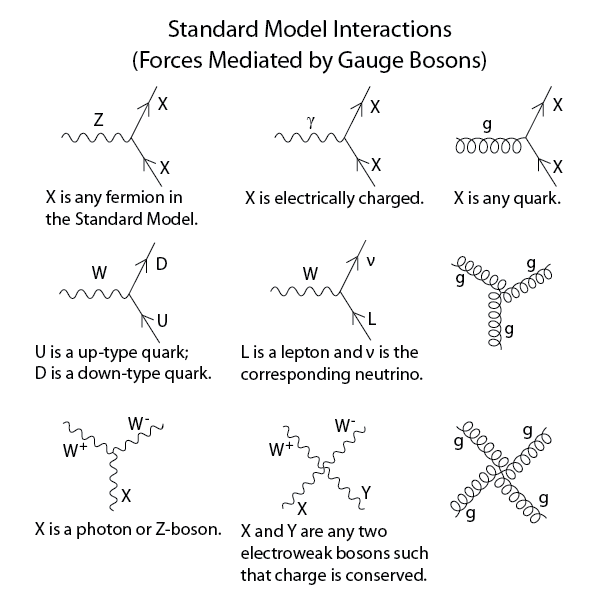
\includegraphics[width=0.7\textwidth]{figures/Phenomenology/Standard_Model_Feynman_Diagram_Vertices.png}
  \caption[Interactions allowed in the SM, excluding those involving the Higgs field]{
    Interactions allowed in the SM, excluding those involving the Higgs field.
    Reproduced from Ref.~\cite{Smith:2646356}.
        }
 \label{fig:SMinteractions}
\end{figure}

The allowed interactions in the SM are illustrated in Fig.~\ref{fig:SMinteractions}. Lines represent
propagating particles, and vertices represent interactions, arising from the
interaction terms in the SM Lagrangian. These illustrations,
known as Feynman diagrams, can be pieced together to give a diagrammatic
picture of a scattering interaction. Fig.~\ref{fig:wz3lfeynman} gives
two illustrative $\cPq\cPq$ interactions---a component of the $\pp$ collision
at the LHC---mediated by the $\PW$ and $\PZ$
bosons, leading to free muons, an electron, and an anti-electron neutrino. 

\begin{figure}[htbp]
  \centering
   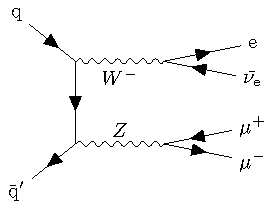
\includegraphics[page=1,width=0.35\textwidth]{figures/FeynmanDiagrams/WZ3lfeynman.pdf}
   \includegraphics[page=2,width=0.35\textwidth]{figures/FeynmanDiagrams/WZ3lfeynman.pdf}
  \caption{
    Feynman diagrams illustrating the $\Pq\Paq\to\mathrm{e}\PAGne\MM$ process,
    proceeding via quark and lepton couplings to the $\PW$ and $\PZ$ bosons.
        }
 \label{fig:wz3lfeynman}
\end{figure}

Feynman diagrams are not just useful as an illustration, they 
represent terms in the perturbative expansion used to model
interactions, specifically, elements of the scattering matrix that 
connects the initial and final state in a scattering experiment. 
So-called Feynman rules
are used to associate the fields and interactions of a diagram with the mathematical
formalism, giving mathematical expressions for the matrix elements
connecting the outgoing particle
four momenta and quantum numbers to the incoming particle properties.
Observables, including the total
rate of production for a final state given the initial state, are dependent
on the square of the scattering matrix elements.

\begin{figure}[htbp]
  \centering
   \includegraphics[page=3,width=0.3\textwidth]{figures/FeynmanDiagrams/WZ3lfeynman.pdf}
   \includegraphics[page=4,width=0.3\textwidth]{figures/FeynmanDiagrams/WZ3lfeynman.pdf}
  \caption{
    Feynman diagrams illustrating the $\Pq\Paq\to\mathrm{e}\PAGne\MM$ process
    with higher-order QCD couplings.
        }
 \label{fig:wz3lfeynmanNLO}
\end{figure}

The diagrams in Fig.~\ref{fig:wz3lfeynman} are not the only possible
set of interactions connecting the $\Pq\Paq$ initial state to the
$\mathrm{e}\PAGne\MM$ state. 
More intricate arrangements of the quark and gluon lines are possible,
as shown in Fig.~\ref{fig:wz3lfeynmanNLO} (left). 
Whereas the diagrams in Fig.~\ref{fig:wz3lfeynman} have four vertices
of fields coupling via the \EW interaction, this diagram has two additional
QCD couplings of the gluon and quarks.
Each vertex contributes and additional factor of the {\EW} or
QCD couplings in the mathematical expression of the scattering matrix element. 
If the coupling term is $\ll$1, the dominant contribution
will come from diagrams such as those shown in Fig.~\ref{fig:wz3lfeynman}, and
it may be possible to neglect the contribution of Fig.~\ref{fig:wz3lfeynmanNLO} (left).
Perturbative calculations rely on this approximation
by restricting a calculation to a maximum ``order'' $\mathcal{O}(\alpha^{n})$ 
in the coupling $\alpha \propto g^2$, by only considering
contributions to a process that have at most a dependence $\alpha^{n}$.

While the diagram in Fig.~\ref{fig:wz3lfeynmanNLO} (right) does lead to a
$\mathrm{e}^{-}\PAGne\MM$ state, it also produces a final-state gluon.
It is tempting to consider this contribution as a separate
process, however, due to the nature of the strong force, such an approach is not favorable experimentally.
Free gluons are not observable, rather, they hadronize into baryons and mesons,
which do not correspond trivially to the radiated partons.
In addition, for gluons radiated at a small angle or low momenta,
it is impossible to experimentally distinguish whether two or one quarks or
gluons are present. For this reason, many leptonic measurements at the LHC
are \emph{inclusive} in the number of associated hadronic particles. That is,
we consider $\pp\to\WZ$ production to include all states producing
the $\mathrm{e}\PAGne\MM$ with any number of associated hadronic objects.

Depending on the process considered and the accuracy needed for a calculation,
neglecting the terms of ``higher order'' may not be appropriate. While the 
Feynman rules are equally applicable for these terms, additional contributions
arise due to the presence of closed loops, as seen for the gluon and quark lines
in Fig.~\ref{fig:wz3lfeynman} (right). These individual diagrams give results
that predict infinite rates, therefore, they cannot correspond to experimental observations.
Fortunately, the situation can be recovered when combining with other diagrams
contributing to the higher-order calculation. A finite contribution can be
isolated and used to describe experimental measurements with incredible accuracy.
Infinite terms remain, but they can be associated with experimentally-established
terms---in particular, the masses and couplings of the theory. This procedure,
known as \emph{renormalization}, is closely connected to the energy scale of the process
and the structure of the fields themselves. In this approach, the coupling constant 
captures the neglected contributions from diagrams contributing at higher perturbative orders,
becoming an effective coupling at the energy scale considered.

\begin{figure}[htbp]
  \centering
   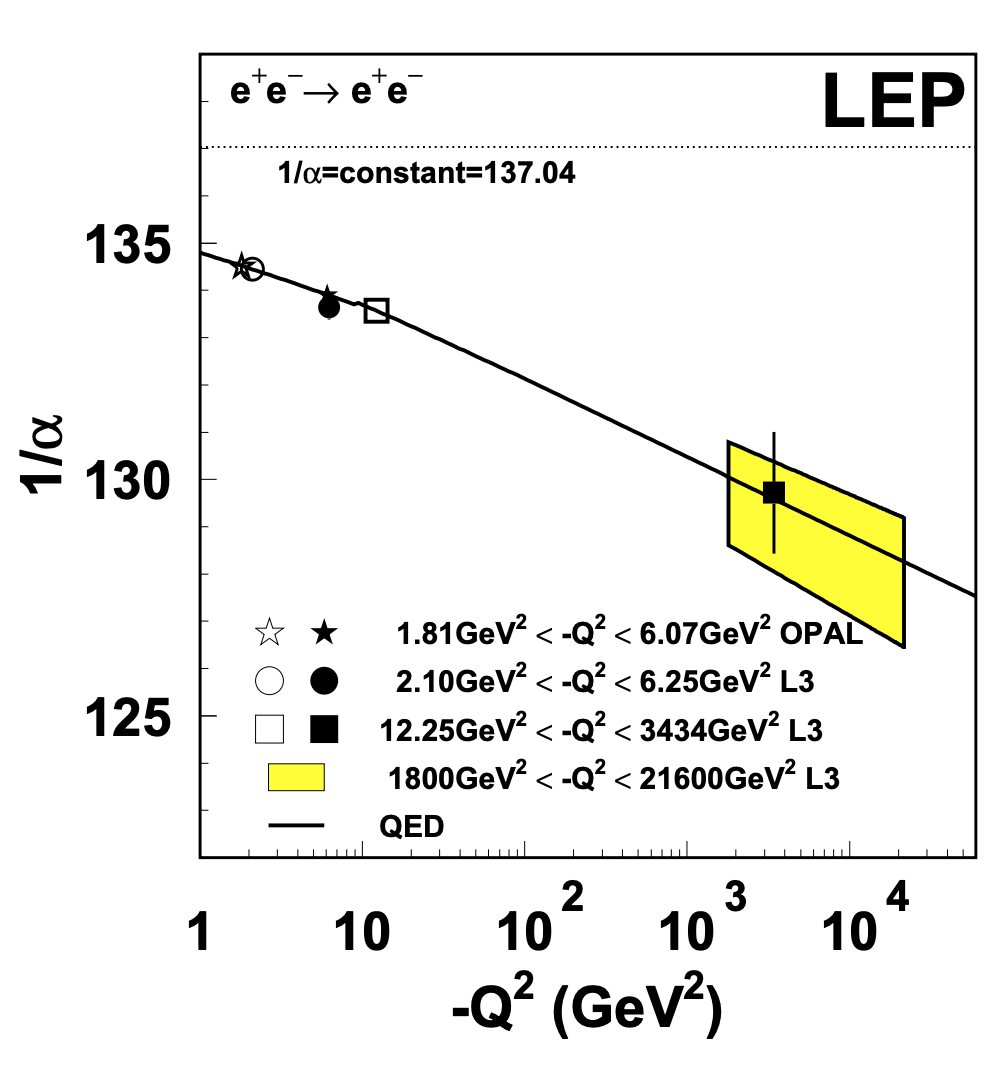
\includegraphics[width=0.39\textwidth]{figures/Phenomenology/alphaRunning.png}
   \raisebox{0.1\height}{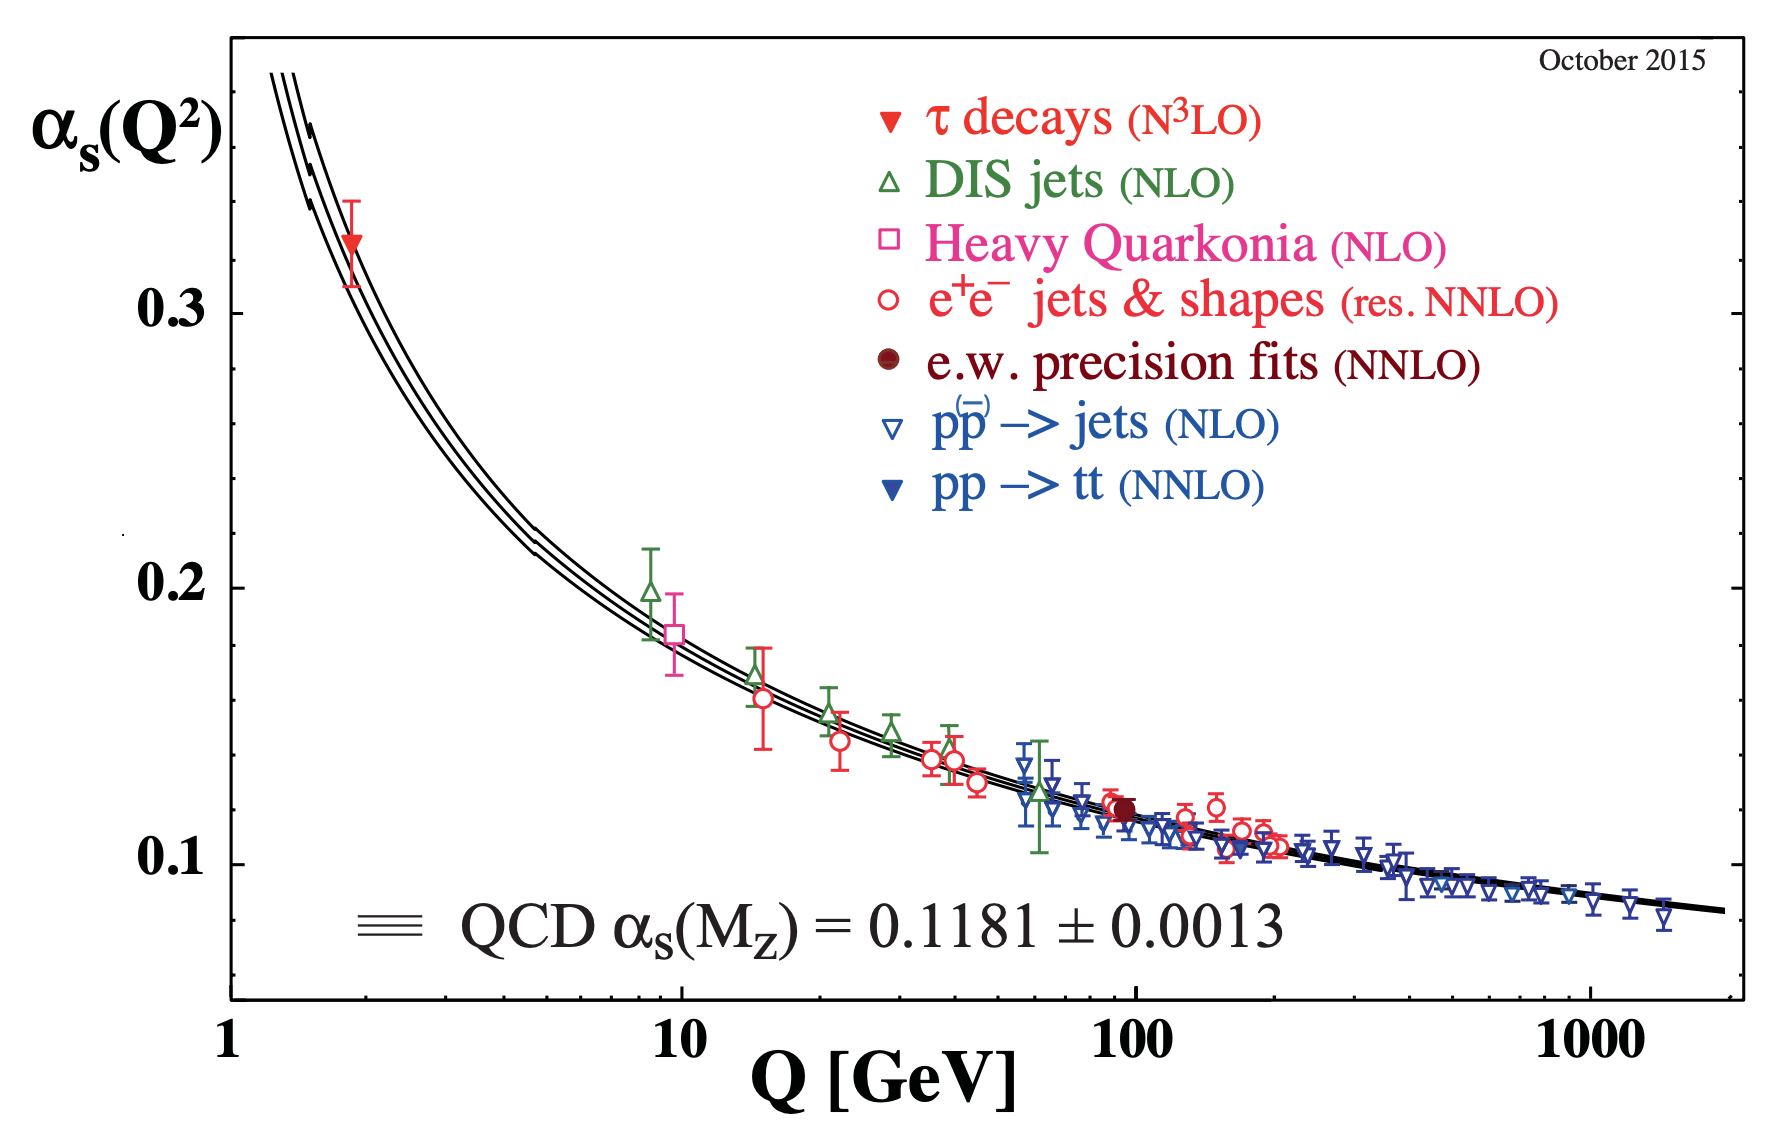
\includegraphics[width=0.59\textwidth]{figures/Phenomenology/alphasRunning.png}}
  \caption[The energy scale dependence of the effective EW and QCD couplings]{
    The energy scale dependence of the effective EW (left, reproduced from Ref.~\cite{Mele:2006ji}) 
    and QCD (right, reproduced from Ref.~\cite{Tanabashi:2018oca}) couplings. The theoretically
    predicted bands and discrete points established experimentally are shown.
  }
  \label{fig:couplings}
\end{figure}

The energy dependence of the effective coupling constants for the 
EW and QCD theories are shown in Fig.~\ref{fig:couplings}.
As shown, the nature of the $\SUthree$ and $\SUtwo$ forces leads to a striking difference
in energy dependence between the two theories: the EW coupling strength increases
with energy, whereas the QCD coupling decreases, leading to the 
confinement of quarks and gluons into bound states, such as the proton and neutron,
at low energies. At the energy scale probed in LHC collisions, the QCD coupling is
sufficiently small for perturbative calculations, however, higher-order corrections
are often significant. The scale dependence of the EW coupling is minimal, so
higher-order EW corrections are often not essential to accurate calculations.
Perturbative calculations are discussed in more detail in Chapter~\ref{ch:simulation}.

\section{The \WZ production at the LHC}

At low energy, the proton can be viewed as a bound state
of the quarks $\cPqu\cPqu\cPqd$. However, at higher energy, the content of the proton
appears more complex. High-energy quarks can radiate gluons, which can split to $\cPq\cPaq$ pairs.
In the high-energy \pp collisions at the LHC, the proton is a source of gluons, and
all flavors of quarks but the heaviest, the top quark.
Therefore, the initial state of fundamental particles in the interactions studied at the LHC is always
composed of quarks and gluons, collectively dubbed ``partons.'' The energy of the colliding 
protons is controlled, but the flavor and energy of the interacting partons can only 
be inferred based on these properties, as discussed in Chapter~\ref{ch:simulation}.

The dominant modes of $\pp\to\WZ\to\threelnu$ 
(were $\ell,\ell'=\mathrm{e},\mu$) production are shown in Fig.~\ref{fig:wz3lfeynman}.
Equivalent diagrams are possible with the $\PW$ and $\PZ$ bosons coupling
to quarks, or the $\PZ$ boson to neutrinos. Many aspects of the processes are similar,
and it is often justified to treat the $\pp\to\WZ$ and $\WZ$ decay to leptons, neutrinos,
or quarks separately. For this reason, we refer to ``$\WZ$ production,'' keeping in mind
that the $\PW$ and $\PZ$ bosons have an extremely short lifetime and are only observable
via their decay products. The results in this thesis exploit the leptonic decay channels,
$\PW^{-}Z\to\EE\mu^{-}\PAGnGm$, 
$\PW^{+}Z\to\EE\mu^{+}\PGnGm$, 
$\PW^{-}Z\to\MM\mathrm{e}^{-}\PGnGm$, and
$\PW^{-}Z\to\MM\mathrm{e}^{+}\PGne$.

Studies of $\WZ$ production at the LHC provide an important test of the SM.
As shown in Fig.~\ref{fig:wz3lfeynman} (right), the process is sensitive to the charged $\PW\PZ\PZ$
coupling, which arises due to the non-Abelian nature of the electroweak
theory, and is exactly predicted in the SM~\cite{Hagiwara:1986vm}. Additional charged
resonances, or other modifications of the \EW sector of the SM, would
modify this process and adjust the rate. Moreover, the process is known
to be sensitive to higher-order corrections~\cite{Grazzini:2016swo}. Measuring this process
with sufficient accuracy to test state-of-the-art calculations, and to 
determine consistency with the SM or uncover hints of new physics, is
of great interest to the LHC experimental program.

As mentioned in the previous section, it is often advantageous to consider
measurements inclusive in the number of hadronic particles. It is possible, however,
to make exclusive measurements, provided that we are careful in how we associate
the number of hadronic objects to the number of partons in a Feynamn diagram.
The solution is to cluster the partons, or hadrons, using algorithms that are
well-behaved for low energy partons. We refer to these clustered hadronic objects as
``jets,'' (\jet) and a close correspondence between experimental measurements and theoretical
predictions has been demonstrated for several so-called jet-clustering algorithms.
The specific algorithms used in this analysis will be discussed in Chapter~\ref{ch:reconstruction}.

The focus of this thesis is the process
$\pp\to\WZjj$, an important subcomponent of the inclusive $\pp\to\WZ$ process
Here, and throughout this thesis, $\WZjj$ refers to $\WZ$ production,
with leptonic decays,
associated with at least two jets in the event, e.g., a final state of $3\ell\nu\jet\jet$.
While it is often useful to relate the $\WZ+2$ partons calculation and the $\WZ+2$ jets (\WZjj)
experimental state, it is important to note that the relationship is most appropriate
when using a common jet clustering algorithm.
The dominant contribution to the $\WZjj$ state is a higher-order correction to the 
diagrams of Fig.~\ref{fig:wz3lfeynman}, where gluons are radiated from the incoming
quarks. Because of the additional
QCD vertices, these diagrams contribute to the \WZjj state at $\mathcal{O}(\alpha_s^{2}\alpha^{2})$,
compared with $\mathcal{O}(\alpha_s^{0}\alpha^{2})$ for the dominant contributions to the $\pp\to\WZ$
process. At this order, contributions from $\cPq\cPg$ and $\cPg\cPg$ initial
states also contribute, slightly enhancing the total $\WZjj$ production rate.

\begin{figure}[htbp]
  \centering
   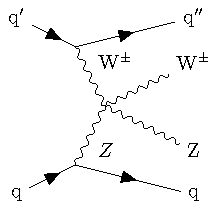
\includegraphics[page=1,width=0.23\textwidth]{figures/FeynmanDiagrams/feynmanEW.pdf}
   \includegraphics[page=2,width=0.23\textwidth]{figures/FeynmanDiagrams/feynmanEW.pdf}
   \includegraphics[page=4,width=0.23\textwidth]{figures/FeynmanDiagrams/feynmanEW.pdf}
   \includegraphics[page=3,width=0.23\textwidth]{figures/FeynmanDiagrams/feynmanEW.pdf}
  \caption[Representative Feynman diagrams for \EWWZ production in the SM]{
    Representative Feynman diagrams for \EWWZ production in the SM,
  including those with quartic \WWZZ interactions (left) and via scattering with the Higgs boson (right).
  }
 \label{fig:feynmanDiagramsVBS}
\end{figure}

Another contribution at $\mathcal{O}(\alpha_s^{0})$ emerges, of
order $\mathcal{O}(\alpha_s^{4})$. 
The subclass of processes with only EW couplings at tree level has a rich
and important phenomenology.
It includes contributions from vector boson scattering (VBS), 
where vector bosons are radiated from the incoming quarks before interacting,
as illustrated in Fig.~\ref{fig:feynmanDiagramsVBS}. 
The VBS processes form a distinct experimental signature characterized by 
the $\PW$ and $\PZ$ bosons with two forward, 
high-momentum jets, arising from the hadronization of two quarks. 
The previously discussed contributions to the \WZjj state that proceed via QCD 
radiation of partons from are referred to as QCD-induced WZjj production (or \QCDWZ).

\section{Probing the electroweak sector through vector boson scattering}

As illustrated in Fig.~\ref{fig:feynmanDiagramsVBS} (right), \EWWZ production 
is sensitive to the quartic couplings of the vector bosons, as well as the 
interactions of the vector bosons and the Higgs boson. Additional interactions
in the \EW sector, such as heavy new scalar Higgs bosons, would lead to additional
contributions, modifying the effective rate of production of \EWWZ events.

The existence of the Higgs boson has strong implications for VBS VV production.
The longitudinally polarized component of the diagrams of Fig.~\ref{fig:feynmanDiagramsVBS} 
that do not involve the Higgs
couplings increase with the scattering energy without bound.
In 1987, an analysis of VBS production of $\PW{+}\PW^{-}$ in $\pp$ collisions
by Lee, Quigg, and Thacker demonstrated that the presence of a scalar boson is necessary to regulate
this component to a finite rate~\cite{Lee:1977yc}.
By analyzing the partial wave amplitudes of the process, they derived a unitary
bound on for the process that stipulated $m_{\PH} \lessapprox 1\TeV$, providing a convincing argument for
the Higgs boson to be discovered at the future LHC. 
While the observed SM Higgs is sufficient to regulate the process, further modifications
could disturb this cancellation, leading to large deviations from the SM predictions.

This thesis presents a measurement of the \EWWZ process under the assumption that
its rate and characteristics are those of the SM prediction. 
We also search for deviations from the SM in both the rate of production of events characteristic
of the \EWWZ process, and in differential distributions sensitive to the scattering energy
of the interaction and the mass of new scalar particles. We interpret the results in terms 
of both explicit models predicting charged Higgs bosons, shown in Fig.~\ref{fig:feynmanNP} (left),
and in the generalized framework of dimension-8 effective field theory, illustrated in
Fig.~\ref{fig:feynmanNP} (right). In this diagram a set of unknown interactions are represented,
which result in a modification of the effective quartic vertices. The charged Higgs 
and EFT models we investigate are complimentary: the former is applicable in a regime
where the collision energy allows the resonant Higgs to be directly produced, whereas
the latter is meaningful when the scale of new physics exceeds the LHC collision energy.
The models we consider are described in more detail in the following sections.

\begin{figure}[htbp]
  \centering
   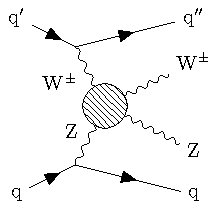
\includegraphics[page=1,width=0.35\textwidth]{figures/FeynmanDiagrams/feynmanNP.pdf}
   \includegraphics[page=2,width=0.35\textwidth]{figures/FeynmanDiagrams/feynmanNP.pdf}
  \caption[Feynman diagrams illustrating hypothetical new physics in the \EWWZ process]{
    Feynman diagrams illustrating hypothetical new physics in the \EWWZ process.
    Charged Higgs production (left) is predicted in many BSM extensions. The aQGC
    approach (right) can be used to parameterize a large class of new interactions modifying the
    \WWZZ process.
        }
 \label{fig:feynmanNP}
\end{figure}

\subsection{Additional Higgs bosons and the Georgi-Machacek model}

In the SM, EWSB is realized by a single isospin doublet scalar field,
as discussed in Section~\ref{sec:ewsb}.
This field is sufficient to give mass to the $\PW$ and $\cPZ$
bosons, while resulting in a scalar $\PH$ boson consistent with the observed
boson with $m_{\PH} = 125\GeV$.  Given the complexity of the fermion sector
of the SM, it is natural to ask if the universe contains a more complex
structure of scalar fields than the single doublet. 
However, SM extensions by arbitrary $\SUtwo$ scalar fields 
are highly constrained by the parameter $\rho \equiv m_\PW^2/m_\PZ^w\cos^2\theta$,
experimentally established to be very close to 1~\cite{Tanabashi:2018oca}.
For a theory with $n$ scalar multiplets
$\phi_i$, with weak isospin $I_i$, weak hypercharge $Y_i$, and vacuum expectation
value $v_i$, $\rho$ is defined in terms of the quantum numbers of the fields
by the following expression at tree level~\cite{Branco:2011iw}
\begin{equation}
  \rho = \sum_{i = 1}^{n} \frac{I_i(I_i+1) - \frac{1}{4}Y_i^2}
              {\frac{1}{2}Y_i^2 v_i} \,,
  \label{eq:rho}
\end{equation}
Extending the scalar sector of the SM by two rather than one doublet satisfies
this expression. This model, known as the Two-Higgs-doublet model (2HDM), has
been extensively studied, in part because the scalar sector of 
many popular theories of supersymmetry have this form.
The 2HDM gives rise to a heavy Higgs boson, a pseudoscalar Higgs boson, and 
charged Higgs bosons $\PH^{\pm}$ in addition to a light SM-like Higgs boson.
In this model, the $\PH^{\pm}$ bosons coupling strongly to the leptons,
and decays to bosons are strongly suppressed in the mass range probed by the LHC~\cite{Arhrib:2016wpw}.

Alternatively, if the Higgs sector of the SM is extended by scalar $\SUtwo$ triplets,
charged Higgs bosons with tree-level couplings to the $\PW$ and $\PZ$ bosons are 
generated by EWSB.
Higgs triplets appear in left-right symmetric~\cite{Pati:1974yy,Mohapatra:1974gc,},
little Higgs~\cite{ArkaniHamed:2002qy,Chang:2003zn,Chang:2003un}, 
and some supersymmetric models~\cite{Garcia-Pepin:2014yfa,Cort:2013foa}.
A simple extension of the SM with Higgs triplets that satisfies experimental
constraints on $\rho$ was proposed by Georgi and Machecek~\cite{Georgi:1985nv}.
In the Georgi Machacek (GM) model, the Higgs sector is extended by a real 
triplet with $Y=0$ and 
a complex triplet with $Y=2$ in addition to the usual SM doublet ($Y =1$). 
After EWSB, this leads to a rich Higgs sector with intriguing phenomenology.
The Higgs sector of the GM has ten physical states that are organized based
on their transformation properties under the approximate global $\SUtwo$ symmetry
of the scalar fields remaining after EWSB, referred to as custodial symmetry~\cite{Sikivie:1980hm}. There are two singlets,
one of which is associated with the observed Higgs boson, a triplet, and 
a fiveplet ($\PH_5^{++}$, $\PH_5^{+}$, $\PH_5^{0}$, $\PH_5^{-}$, $\PH_5^{--}$) that
is fermiophobic. If the mass of the triplet states is greater than the
mass of the fiveplet, the only production mechanism for $\PH^{\pm}$ at the LHC
is vector boson fusion (VBF, shown in Fig.~\ref{fig:feynmanNP}, left). The production cross section is proportional to the variable
$s_{\PH}^2 \equiv \sin^2{\theta_{\PH}}$, where $\sin{\theta_{\PH}} = 2\sqrt{2}v_{\chi}/v$,
the ratio
of the vacuum expectation value (vev) of the triplet fields to the SM vev. 
The $\WZjj$ state probed in this thesis is well-suited for further probes of this model, 
which is significantly less constrained than those charged Higgs with predominantly
leptonic decays.

\subsection{Generalizing new interactions with effective field theory}

Explicit models of charged Higgs production, such as those
discussed in the previous section, provide a well-motivated set of characteristics
to exploit in searches for deviations from the SM. 
In such a paradigm, expectations
about the underlying structure of the theory allow explicit relationships
between independent measurements to be drawn. 
However, when results favor
the SM to a proposed extension, it may be useful to cast a wider net, in search
of more subtle or more exotic extensions. Furthermore, if the mass scale
of new physics---such as a heavy charged Higgs bosons---exceeds the range 
directly probed by 13\TeV \pp collisions, a broad characterization of a deviation,
or lack thereof, may be more meaningful than sensitivity to a particular model.

Effective field theory (EFT) is well suited for a broad characterization
of new physics at a high energy scale. In EFT, the SM is assumed to describe the
field content of the universe below some scale $\Lambda$. 
Additional fields may exist, but they are only directly accessible (e.g., 
resonant production at a collider) above $\Lambda$. Below this scale,
their effect on the low-energy world can be parameterized in terms of the known
SM field content. These interactions are realized by adding additional terms
to the SM Lagrangian, built from the SM fields, of mass dimension $>$4. In order
to restore calculability of these interactions, a dimensionful coupling must also,
which is proportional to the inverse of the scale $\Lambda$.

The bottom-up approach to EFT described here, in which
new interactions are parameterized in terms of the low-energy field content,
is useful because it is consistent with a top down approach, where the low-energy behavior is extracted
from a known full theory~\cite{Kaplan:2005es}. The most well-known example of this is the Fermi theory
of the weak decay $\mathrm{n}\to\PAp\mathrm{e}^{-}\PAGne$. 
A low energy description, in which the leptons, quarks, and neutrinos couple
directly in a four-fermion interaction was original proposed by Fermi without knowledge
of the underlying theory. 
In the full \EW theory, the interaction between
a $\cPqd$ quark of the neutron and an electron is mediated by the $\PW^{-}$ boson,
through $\cPqd\PW^{-}\cPqu$ and $\mathrm{e}^{-}\PW^{-}\PAGne$ couplings of the EW theory.
Because the momentum exchange $p$ of the interaction is on the MeV scale, whereas 
$m_{\PW} = 80.4\GeV$, the full expression for the interaction can be expanded in 
terms of the ratio $p/M$, to derive an approximate theory valid at low energy
with the effective coupling $G_{F} = \sqrt{s}g^2/8m_{\PW}^2$ of Fermi's theory.
In this sense, the low-energy EFT gives insight gives useful predictions within
its energy regime and provides insight into the nature of the full theory.

In this analysis, we consider a set of dimension-8 EFT operators sensitive
to the quartic interactions of the $\PW$, $\PZ$, and $\gamma$. Because an alternative,
largely historical, approach to parametrizing these interactions involves
directly modifying the coupling terms in the Lagrangian, we refer to this 
as a search for anomalous quartic gauge couplings (aQGC). Similarly, anomalous triple gauge
couplings (aTGC), probed in inclusive $\WZ$ production,
can be parameterized by dimension-6 operators. 

The set of operators considered in this analysis
are shown in Equation~\ref{eq:aqgc}.
\begin{equation}
  \begin{aligned}
    \mathcal{L}_\text{S0} = & \frac{f_\text{S0}}{\Lambda^4} \left[(D_\mu \Phi)^\dagger(D_\nu \Phi)\right]\times\left[(D^\mu \Phi)^\dagger(D^\nu \Phi)\right] \\
    \mathcal{L}_\text{S1} = & \frac{f_\text{S1}}{\Lambda^4} \left[(D_\mu \Phi)^\dagger(D^\mu \Phi)\right]\times\left[(D_\nu \Phi)^\dagger(D^\nu \Phi)\right] \\
    \mathcal{L}_\text{T0} = & \frac{f_\text{T0}}{\Lambda^4} \text{Tr}\left[\hat{W}_{\mu\nu} \hat{W}^{\mu\nu}\right] \times \text{Tr}\left[\hat{W}_{\alpha\beta} \hat{W}^{\alpha\beta}\right] \\
    \mathcal{L}_\text{T1} = & \frac{f_\text{T1}}{\Lambda^4} \text{Tr}\left[\hat{W}_{\alpha\nu} \hat{W}^{\mu\beta}\right] \times \text{Tr}\left[\hat{W}_{\mu\beta} \hat{W}^{\alpha\nu}\right] \\
    \mathcal{L}_\text{T2} = & \frac{f_\text{T2}}{\Lambda^4} \text{Tr}\left[\hat{W}_{\alpha\mu} \hat{W}^{\mu\beta}\right] \times \text{Tr}\left[\hat{W}_{\beta\nu} \hat{W}^{\nu\alpha}\right] \\
    \mathcal{L}_\text{M0} = & \frac{f_\text{M1}}{\Lambda^4} \left[(D_\mu \Phi)^\dagger(D_\nu \Phi)\right]\times\left[(D^\mu \Phi)^\dagger(D^\nu \Phi)\right] \\
    \mathcal{L}_\text{M1} = & \frac{f_\text{M1}}{\Lambda^4} \left[(D_\mu \Phi)^\dagger(D^\mu \Phi)\right]\times\left[(D_\nu \Phi)^\dagger(D^\nu \Phi)\right]
  \end{aligned}
  \label{eq:aqgcOperators}
\end{equation}
Here
\begin{equation}
  \hat{W}_{\mu\nu} = \sum_j W_{\mu\nu}^j \frac{\sigma^j}{2}\,,
\end{equation}
where $W_{\mu\nu}$ are the $\SUtwo_{L}$ fields before EWSB
and the values $f_{\text{S}i}$, $f_{\text{T}i}$, and $f_{\text{M}i}$ are
dimensionless couplings to the dimension-8 operators.

The operators probed are a subset of those outlined in 
Ref.~\cite{Eboli:2006wa}, which proposes
nine independent dimension-eight operators that
assume the $\SUtwo\times\Uone$ symmetry of the EW gauge sector as well as
the presence of an SM Higgs boson. All operators are
charge conjugation and parity conserving.
The $\mathcal{L}_\text{Si}$ operators
are a function of the scalar Higgs field. The $\mathcal{L}_\text{Ti}$ operators are
functions of the gauge fields, and the $\mathcal{L}_\text{Ti}$ operators are
built from a mix of the scalar and gauge fields. The quartic gauge
coupling can be expressed in terms of these operators as 
\begin{equation}
\mathcal{L}_{quartic} = f_\text{S0}\mathcal{L}_\text{S0} + f_\text{S1}\mathcal{L}_\text{S1} \,.
\end{equation}
With $f_\text{S0} = -f_\text{S1} = f$, non-zero values of $f$ give a rescaling
of the SM coupling by $(1+fv^{4}/8)$.

\section{Previous results}

\subsection{Measurements of \WZ production}

The $\WZ$ production was first observed
in $\Pp\PAp$ collisions by the CDF~\cite{Aaltonen:2012vu,Abulencia:2007tu} 
and D0~\cite{Abazov:2012cj} Collaborations at the Tevatron in 2006. 
The inclusive \WZ production cross section in \pp collisions 
has been measured in the leptonic decay modes by the ATLAS and CMS Collaborations 
at 7, 8, and $13\TeV$~\cite{Aad:2012twa,Aad:2016ett,Aaboud:2016yus,Aaboud:2019gxl,Khachatryan:2016tgp,Khachatryan:2016poo}, 
A summary of these measurements is 
shown in Fig.~\ref{fig:WZxsecSqrts}. The summarized experimental results are obtained
by measuring $\pp\to\WZ\to\ell'\ell'\ell\nu$ process, corrected for the 
independently-measured leptonic branching ratios (the percentage of events with
$\PW\to\ell\nu$ and $\PZ\to\ell'\ell'$ to all other decay channels), to obtain a total
rate for the process $\pp\to\WZ$. Theoretical predictions are shown at 
next-to-leading order (NLO) in QCD, in which all contributions to the process 
up to $\alpha^{2}\alpha_s$ are considered in the calculation,
and at next-to-next-to-leading order (NNLO), which considers contributions up 
to $\alpha^{2}\alpha_s^{2}$. The predictions are obtained using the programs
MCFM~\cite{Campbell:2011bn,Campbell:2015qma} and MATRIX~\cite{Grazzini:2016swo,Grazzini:2017mhc}.
The data exhibit a slight preference for the higher-order prediction, demonstrating
the importance of both high-precision measurements and calculations.

\begin{figure}[htbp]
  \centering
   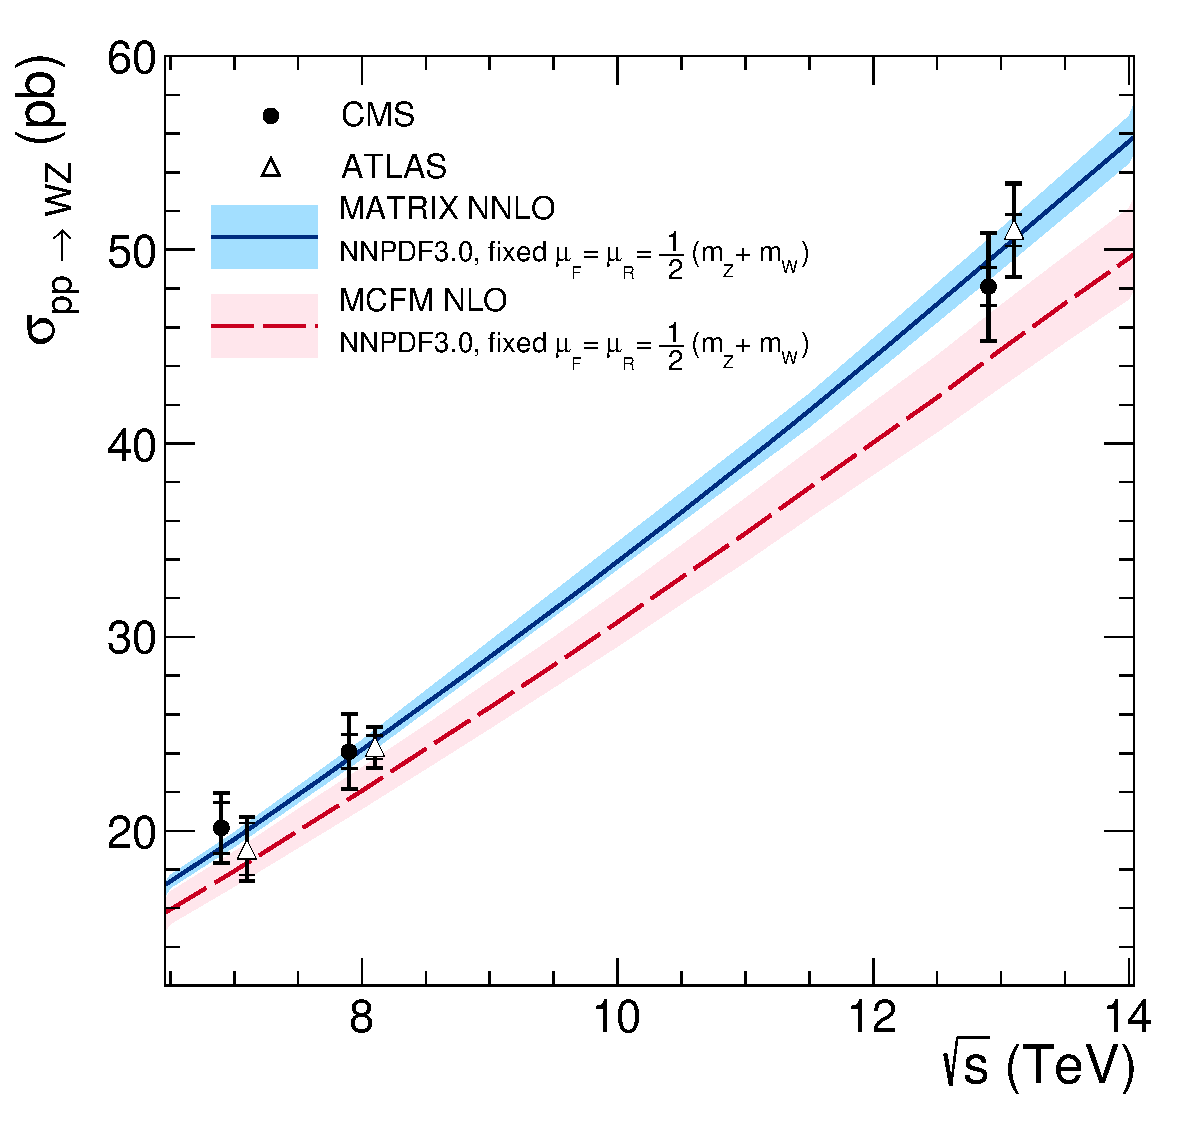
\includegraphics[width=0.8\textwidth]{figures/Phenomenology/WZCrossSection_preliminary_2019-02-23.pdf}
  \caption{
    The measured $\pp\to\WZ$ production cross sections at 7, 8, and 13\TeV compared with
    theoretical predictions at NLO and NNLO in QCD.
        }
 \label{fig:WZxsecSqrts}
\end{figure}


\subsection{Measurements of $\WZjj$ production and electroweak \WZ production}

Fig.~\ref{fig:WZnJets} shows the distribution of the number of jets associated with
the selected $\ell\ell\ell'\nu$ state in data collected by the CMS experiment
in 2015. This analysis, the first measurement of the $\WZ$ process at 13\TeV,
was a critical first step towards the $\WZjj$
studies presented in this thesis. The expected contribution from the $\WZ$
process, along with the estimated backgrounds, are seen to be in good agreement
with the observed data. This studies of this thesis are performed with
a higher-luminosity data set, in order to exploit the kinematics variables of the selected
jets to isolate the $\EWWZ$ and new physics contributions.

\begin{figure}[htbp]
  \centering
   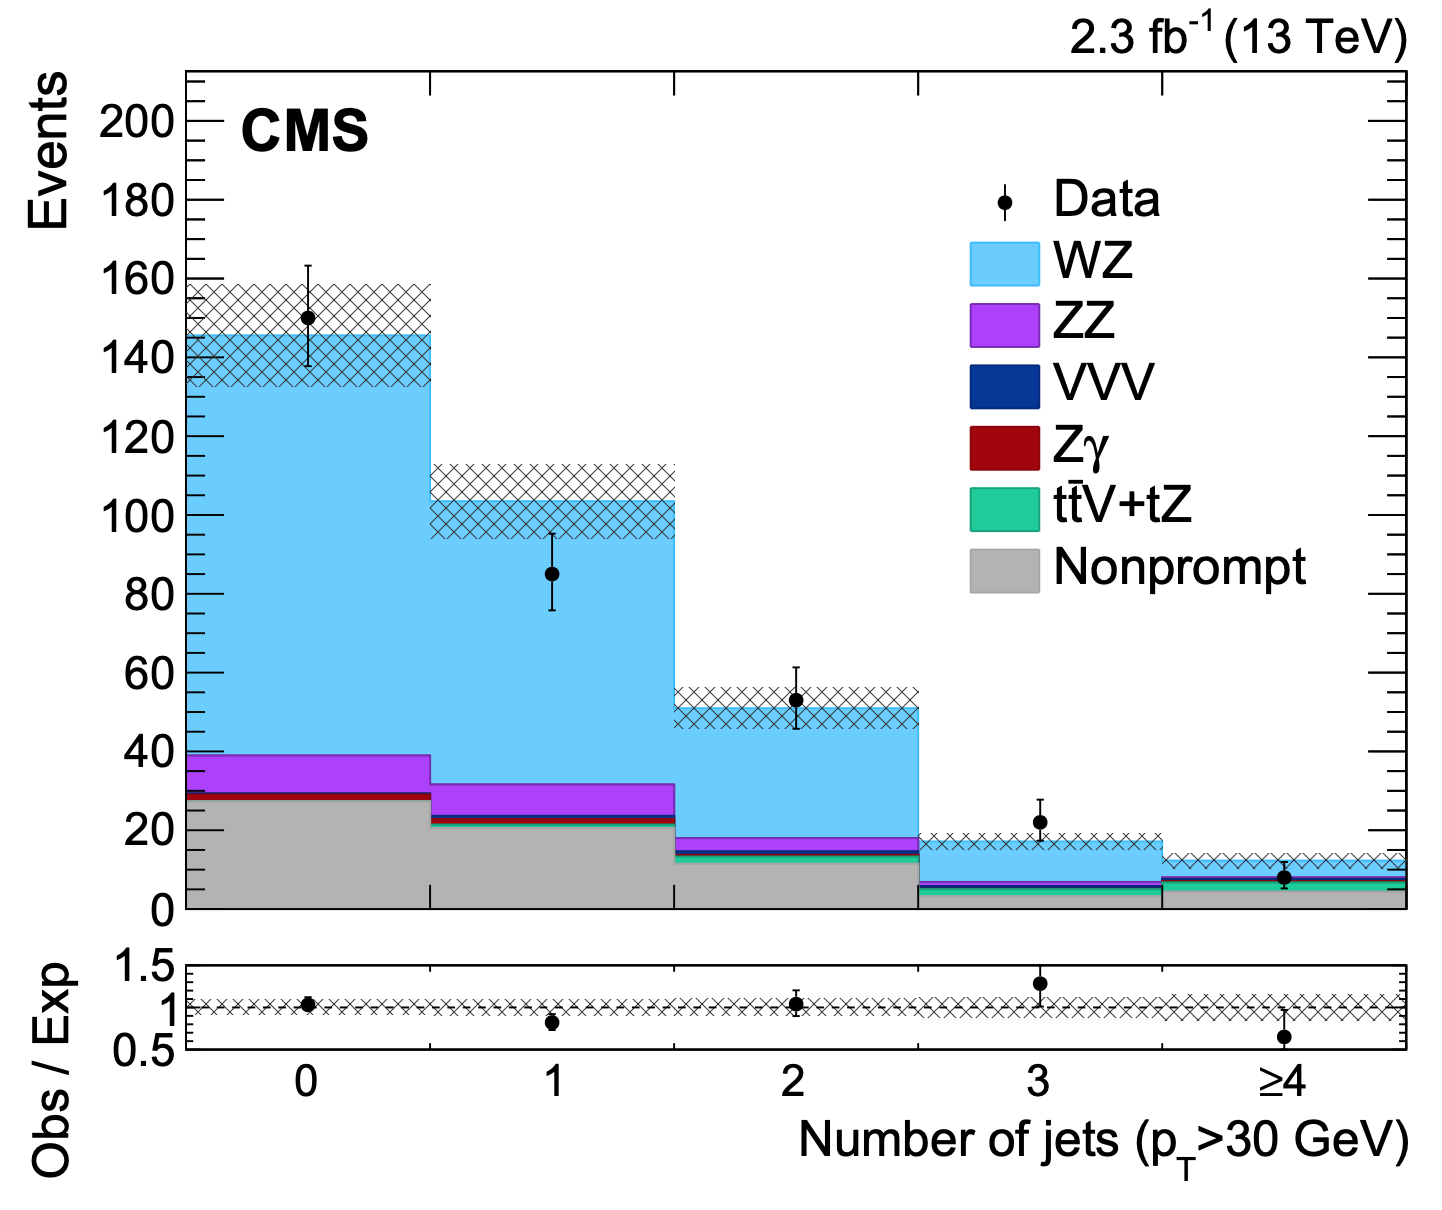
\includegraphics[width=0.6\textwidth]{figures/Phenomenology/WZnJets2015.png}
  \caption{
    The number of jets in selected $\ell'\ell'\ell\nu$ events
    for the observed data and the expected $\WZ$ signal and background 
    contributions using 2.3\fbinv of data collected by the CMS experiment in
    2015~\cite{Khachatryan:2016tgp}.
        }
 \label{fig:WZnJets}
\end{figure}

The first studies of VBS production of pairs of massive vector 
bosons---termed diboson production, or VV production, where $\text{V}=\PW,\PZ$---were 
performed using in the $\pp\to\Wpm\Wpm\to\ell^{\pm}\nu\ell'^{\pm}\nu'$
channel at 8\TeV~\cite{Khachatryan:2014sta,Aad:2014zda,Aaboud:2016ffv}.
This channel is advantageous at the LHC, because, contrary to all other VV states,
the {\EW}-induced production dominates the QCD-induced production. The first
measurement of VBS production of a massive VV state with statistical significance
exceeding 3.0 standard deviations ($\sigma$) is presented by the ATLAS Collaboration 
in the analysis of Ref.~\cite{Aad:2014zda}.
The \EWWZ production was also studied at 8\TeV by the ATLAS Collaboration,
which places upper limits on the production cross section in Ref.~\cite{Aad:2016ett},
and the CMS Collaboration, which reports a \WZjj cross section in a region
sensitive to \EWWZ production in Ref.~\cite{Khachatryan:2014sta}.

Studies of \EW $\Wpm\Wpm$ have recently been performed by the CMS and ATLAS Collaborations at 
13\TeV~\cite{Sirunyan:2017ret,ATLAS-CONF-2018-030}.
The first measurement of \EW VV production with a statistical significance greater than 5 standard 
deviations, considered the standard for discovery of new processes by the experimental particle 
physics community, is presented by the CMS Collaboration in Ref.~\cite{Sirunyan:2017fvv}. A subsequent study
performed by the ATLAS Collaboration~\cite{ATLAS-CONF-2018-030} reports a comparable observation for the process.
The first study of the \EW VV production with a $\PZ$ boson was performed in the $\pp\to\ZZ$ channel
by the CMS Collaboration~\cite{Sirunyan:2017jej}. The observed statistical significance of the 
measurement is $2.7\sigma$ with $1.9\sigma$ expected in the SM.

The analysis of this thesis, submitted for publication to the journal \emph{Physics Letters B}~\cite{Sirunyan:2019ksz},
is the first study of \EWWZ production performed by the CMS.
An analysis using a comparable data set of $\pp$ collisions at 13\TeV
has also been submitted to the journal \emph{Physics Letters B} by the ATLAS collaboration~\cite{Aaboud:2018ddq}.
The ATLAS analysis reports and observation of the \EWWZ process with observed statistical significance of
$5.3\sigma$, with $3.4\sigma$ expected in the SM.


\subsection{Searches for anomalous quartic gauge couplings}

Anomalous triple and quartic gauge couplings were studied with
measurements of $\PW\PW$ and $\PW\PW\gamma$ production in electron-positron collisions
at the LEP Collider at CERN by the ALEPH, DELPHI, L3, and OPAL Collaborations~\cite{LEP-2}.
These processes are sensitive to the triple vector boson couplings
$\WWZ$ and $\PW\PW\gamma$, and the quartic couplings $\PW\PW\gamma\gamma$
and $\PW\PW\PZ\gamma$. The production rate and angular distributions of the decay
products of the vector bosons in these states were used to derive values 
of the triple and quartic couplings. No deviations were observed from the 
predictions of the SM were observed.
Limits on the anomalous triple gauge coupling \WWZ~\cite{Hagiwara:1989mx} 
were also presented by CDF and D0 collaboration in 
Ref.~\cite{Aaltonen:2012vu,Abazov:2012ze}, followed by studies performed by the ATLAS and CMS Collaborations in 
Refs.~\cite{Aad:2016ett,Khachatryan:2016poo}. 

Experimental sensitivity to the quartic coupling \WWZZ 
was first achieved at the LHC.
In pp collisions, quartic WZ interactions are accessible through 
VBS \VV production or trough triple vector boson production (\VVV).
Constraints on the deviations of quartic couplings from the SM prediction in
WZ events with at least two jets were first
presented by the ATLAS collaboration at 8 TeV~\cite{Aad:2016ett}. This thesis
reports the first study of aQGCs in the \WZ channel at 13\TeV.

\begin{figure}[htbp]
  \centering
   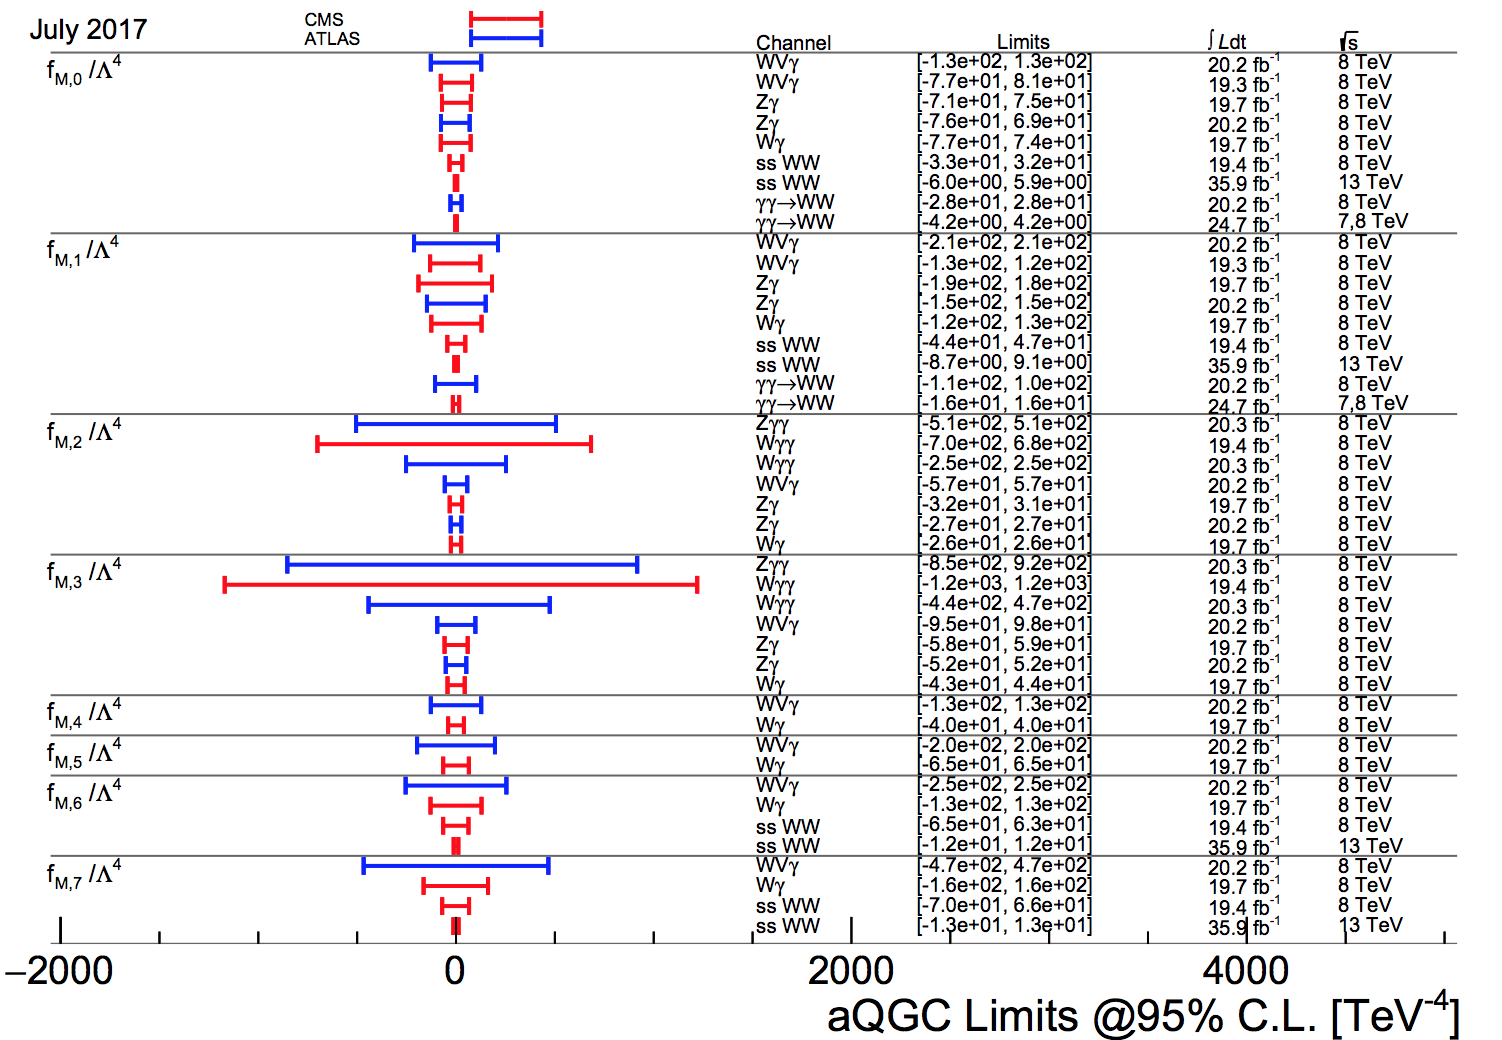
\includegraphics[width=0.95\textwidth]{figures/Phenomenology/FM0_limits_Jun2017.png}
  \caption{
    Constraints on the parameters f$_{\text{Mi}}/\Lambda^4$ for dimension-8 EFT
    operators from the CMS and ATLAS experiments.
        }
 \label{fig:aQGCs}
\end{figure}

Fig.~\ref{fig:aQGCs} illustrates the constraints on the operator parameters
and scale of new physics for the dimension-8 quartic operators
$\mathcal{L}_{\text{T}i}$ from previous studies by the ATLAS and CMS Collaborations.
The most sensitive measurements are those performed in the $\Wpm\Wpm$ channel
reported in Ref.~\cite{Sirunyan:2017ret} and in the $\ZZ$ channel, reported in Ref.~\cite{Sirunyan:2017jej}.

\subsection{Searches for charged Higgs production via vector boson fusion}

The first studies of the production of charged Higgs bosons produced via VBF
and decaying to $\WZ$ at the LHC were performed by the ATLAS Collaboration
at 8~\TeV~\cite{Aad:2015nfa}. The analysis exploited the decay channel
$\Wpm\to\cPq\cPaq'$, $\PZ\to\ell\ell$ 
to place the first direct production constraints on the GM model, as well as model-independent
limits on the production of a narrow-width charged Higgs produced via VBF.
The CMS Collaboration performed the first study of the VBF $\PH^{\pm}$ 
exploiting the leptonic decay channel $\WZ\to\ell\ell\ell'\nu$,
using $15.2\fbinv$ of data collected at $13\TeV$~\cite{Sirunyan:2017sbn}.
The ATLAS Collaboration recently performed an analysis of the same channel
using the data delivered by the LHC in 2016, corresponding to $36.1\fbinv$~\cite{Aaboud:2018ohp},
extending the constraints of the previous CMS analysis.
A local excess of events over the SM prediction at a resonance mass of
around 450\GeV was suggested by this analysis, with a global significance
of $1.9\sigma$ when interpreted in the GM model.
The analysis presented in this thesis extends the results of the previous CMS study, 
and is comparable to the recent study by the ATLAS Collaboration.

\begin{figure}[htbp]
  \centering
   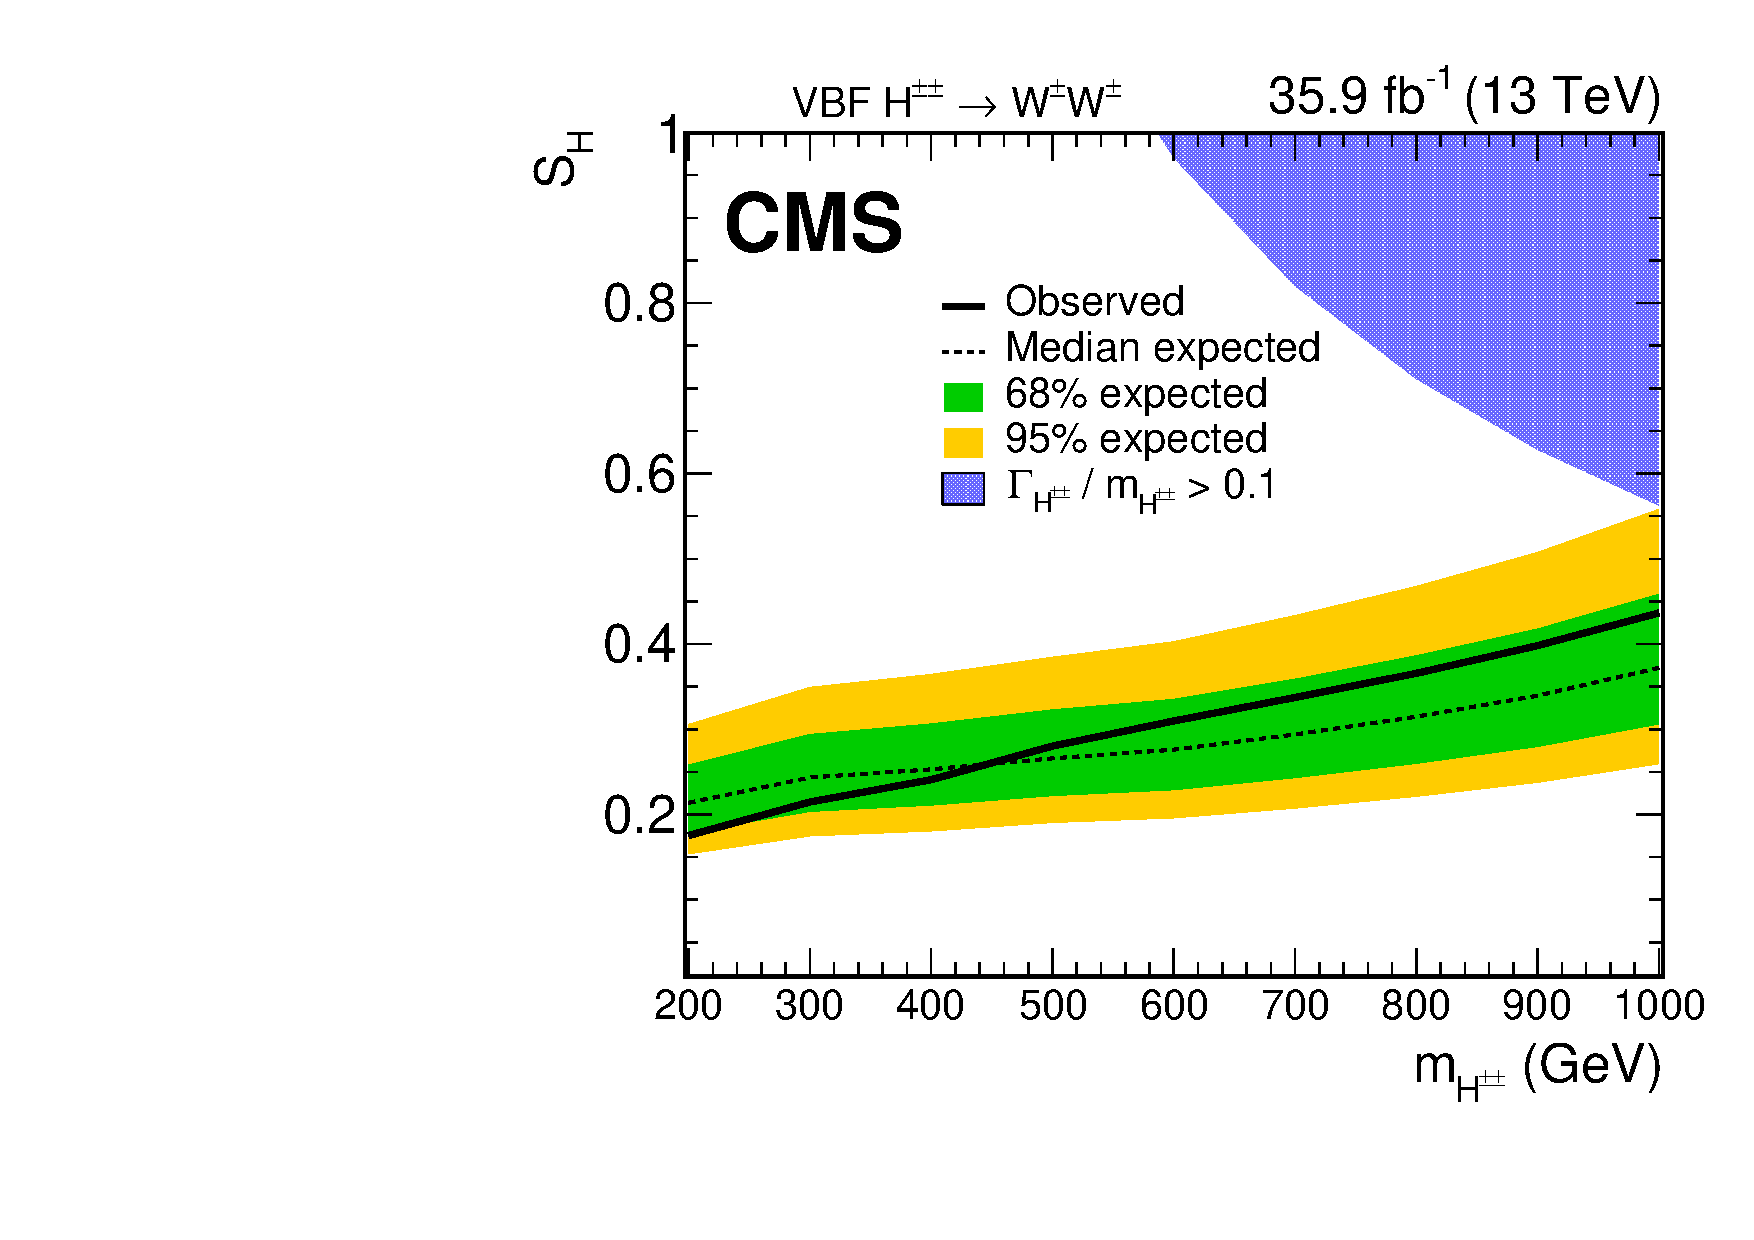
\includegraphics[width=0.44\textwidth]{figures/Phenomenology/CMS-SMP-17-004_Figure_003-b.pdf}
   \raisebox{0.08\height}{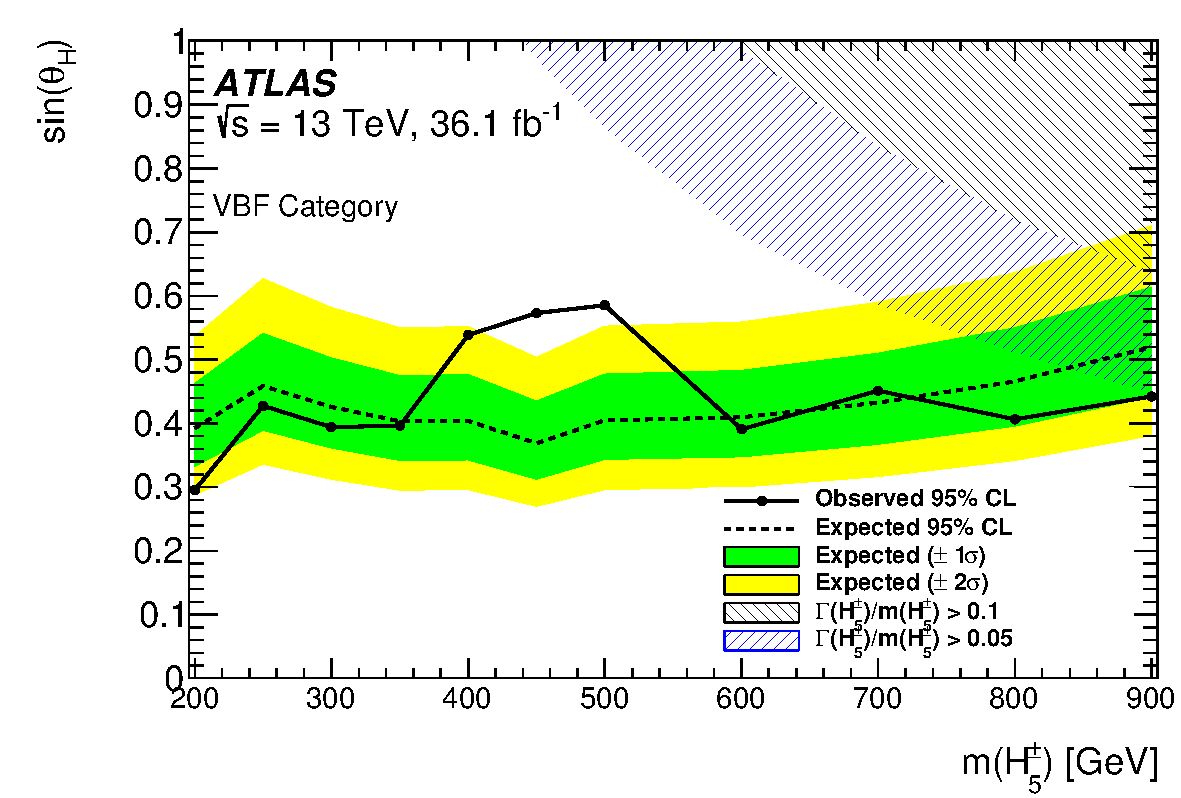
\includegraphics[width=0.54\textwidth]{figures/Phenomenology/ATLAS-EXOT-2016-11_fig_07b.pdf}}
  \caption{
    Limits on production of doubly charged (left, from Ref.~\cite{Sirunyan:2017ret}) 
    and charged Higgs bosons (right, from Ref.~\cite{Aaboud:2018ohp}) in the H5plane defined by the GM model.
        }
 \label{fig:GeorgiMachacekLimits}
\end{figure}

Members of the custodial fiveplet in the GM model have a common mass $m_{\PH^{5}}$.
Therefore, limits on doubly charged Higgs bosons $\PH^{\pm\pm}$
are complementary to those obtained for $\PH^{\pm}$ production when interpreted under this model. 
The ATLAS and CMS
Collaborations have studied $\PH^{\pm\pm}$ production with decays to same-sign
$\PW$ bosons at 8\TeV~\cite{Aad:2014zda,Khachatryan:2014sta}, and the CMS Collaboration has presented
constraints at 13\TeV~\cite{Sirunyan:2017ret}. 
The constraints on the VBF production of $\PH^{\pm}$ in the GM model from Ref.~\cite{Aaboud:2018ohp}
and for $\PH^{\pm\pm}$ from Ref.~\cite{Sirunyan:2017ret} are shown in Fig.~\ref{fig:GeorgiMachacekLimits}.
The limits are presented in terms of $s_{\PH}^2$ and the mass of the $\PH^{\pm}$ or $\PH^{\pm\pm}$
boson, which defines the ``H5plane'' proposed by the LHC Higgs Cross Sections Working Group in Ref.~\cite{deFlorian:2016spz}.
The H5plane is defined with the assumptions that the triplet mass is greater than the 
fiveplet mass and that the parameters of the model allow perturbative calculations. 
Additional constraints on the GM model arise from studies of $\cPqb$ hadron decay
and heavy Higgs boson searches, which are impacted by contributions from additional
Higgs bosons contributing in loop diagrams, but these constraints are exceeded
by the direct measurements discussed here. Global fits of the direct and indirect
constraints on the GM model can be found in Ref.~\cite{Chiang:2018cgb}.

\section{Motivation and content of this result}
The work presented in this thesis
has two related motivations: performing a measurement of a rare
process predicted by the SM, and searching for signs of 
BSM physics in a channel and topology sensitive to modifications of
the EW sector of the SM.
Characterizing the self-interactions of the vector bosons is an important
step to understanding the self-consistency of the SM, and a useful probe
of possible deviations from its predictions. Because the production of events
with multiple vector bosons in the final state
requires collisions with a high center of mass energy, the LHC has
the potential to explore these states in more depth 
than previously achieved.

We perform complementary interpretations of the
observed data and its consistency with the prediction of the SM or signs 
of new physics. In particular, we measure

\begin{itemize}
  \item The total production rate of $\PW\PZ\jet\jet \rightarrow 3\ell\nu\jet\jet$ in
    fiducial regions with enhanced contributions from \EWWZ production
  \item The consistency of the \EWWZ production rate
    with the SM prediction and the statistical significance at which this rate
    can be established as non-zero.
\end{itemize}

We also place constraints on hypothetical new physics using the kinematic
distributions of selected \WZjj events with a VBS topology. 
These processes would be characterized by and excess of VBS \WZ events
with high $m_{\WZ}$, due to the modifications of the quartic VVVV interaction
in a manner sensitive to the scattering energy.
We place limits on the production and model parameters of

\begin{itemize}
  \item Charged Higgs bosons, in a model-independent manner (assuming
    a small $\PH^{\pm}$ width) and in the Georgi-Machacek model.
  \item Anomalous quartic gauge couplings, using the language of
    dimension-eight effective field theory.
\end{itemize}

\bibliographystyle{JHEP}
\bibliography{bibliography}
\end{document}
